% Documento simplificado para una tesis tipo MIT
% Versión más simple con explicaciones contextuales

\documentclass[11pt]{report} % Clase de documento adecuada para tesis

% Paquetes esenciales
\usepackage[letterpaper, margin=1in]{geometry} % Configuración de márgenes
\usepackage{graphicx} % Paquete para incluir gráficos
\usepackage{amsmath} % Paquete para ecuaciones matemáticas avanzadas
\usepackage{amssymb} % Símbolos matemáticos adicionales
\usepackage{setspace} % Espaciado entre líneas
\usepackage{titlesec} % Personalizar los títulos de secciones
\usepackage[hidelinks]{hyperref}
\usepackage{url}
\usepackage{subcaption}
\usepackage{float}

% Eliminar el título automático de thebibliography
\renewcommand{\bibname}{}


% Información de la portada
\title{Charging Station System for swarming drones} % Título de la tesis
\author{José Alberto Castro Villasana \and José Eduardo Castro Villasana \and Ana Bárbara Quintero García} % Nombres de los autores
\date{Diciembre 2024} % Fecha de presentación

\begin{document}

% Portada
\begin{titlepage}
    \centering
    \vspace*{1cm}
    
    {\Huge\textbf{Charging Station System for swarming drones}} % Título en grande
    
    \vspace{2.5cm} % Espacio adicional para centrar mejor
    {\Large\textbf{José Alberto Castro Villasana, José Eduardo Castro Villasana, Ana Bárbara Quintero García}} % Nombres de los autores
    
    \vfill
    
    {\large\textbf{Una Tesis presentada a la Facultad de Ingeniería}} % Información sobre la presentación
    {\large\textbf{en Conformidad con los Requisitos para el Grado de:}} % Información sobre la presentación
    
    \vspace{0.2cm}
    {\large\textbf{Ingeniero en Tecnologías Electrónicas y Robótica, Ingeniero en Mecatrónica}} % Información sobre la presentación
    
    \vspace{2cm}
    
    
\includegraphics[width=0.4\textwidth]{pictures/logo_udem.png} % Logo de la institución
    
    \vspace{2cm}
    
    {\large\textbf{Universidad de Monterrey}}

    \vspace{0.2cm}
    {\large\text{ Departamento de Ingeniería y Tecnologías }}

    \vspace{0.2cm}
    {\large\text{San Pedro Garza García, México}} % Institución y departamento
    
    \vspace{1.5cm}
    {\large\textbf{November 30th 2024}} % Fecha de presentación
    
    \vfill
    {\large\textbf{Advisor:} \text{Fermín Castro Aragón}} % Información del asesor
    
\end{titlepage}

% Índice
\tableofcontents
\newpage

% Espaciado entre líneas
\onehalfspacing% Espaciado de 1.5 líneas para mejor legibilidad

% Llamar a capítulos almacenados en archivos externos
\chapter{Introduction} % Capítulo de introducción
% Introducción para la tesis
% Documento independiente para la introducción

\section{Contexto General y Motivación}

\subsection{Contexto del Problema}

En los últimos años, los drones han evolucionado para convertirse en herramientas esenciales en una amplia gama de industrias. Estos vehículos aéreos no tripulados varían en tamaño y capacidad, pero comparten la característica de acceder a áreas difíciles o peligrosas, lo que ha impulsado su uso en sectores como la inspección de infraestructuras, la agricultura de precisión y las operaciones de vigilancia y seguridad. A nivel comercial, los drones están diseñados para realizar tareas repetitivas de manera autónoma, lo que ha revolucionado la eficiencia en dichas áreas.

En el ámbito de la inspección de infraestructuras, los drones son utilizados para monitorear y evaluar el estado de torres eléctricas, aerogeneradores, líneas de transmisión y otras construcciones críticas, permitiendo detectar fallos estructurales sin la necesidad de exponer a los trabajadores a riesgos innecesarios \cite{cite1}. En agricultura, los drones facilitan la gestión de cultivos, monitoreo de riego y la topografía, lo que permite a los agricultores optimizar la productividad y reducir costos operativos \cite{cite2}. En vigilancia y seguridad, se emplean para monitorear incendios forestales, realizar labores de seguridad fronteriza y evaluar daños tras desastres naturales \cite{cite3}.

A pesar de sus múltiples ventajas, uno de los mayores desafíos en la operación continua de drones es la duración limitada de la batería. En aplicaciones profesionales, los drones suelen tener una autonomía de vuelo entre 20 y 30 minutos, lo cual resulta insuficiente para operaciones prolongadas como la inspección de grandes áreas o la vigilancia a largo plazo \cite{cite4}. Además, las condiciones climáticas adversas pueden afectar significativamente el rendimiento y estabilidad de los drones en vuelo, lo que limita aún más su capacidad operativa \cite{cite5}. Estos factores hacen necesario interrumpir las operaciones para recargar las baterías, lo cual afecta tanto la eficiencia como los costos operativos.

Para abordar esta limitación, se han diseñado estaciones de carga automáticas que permiten recargar las baterías sin intervención humana. Sin embargo, las estaciones actuales presentan varios inconvenientes: la mayoría no están diseñadas para gestionar múltiples drones de manera simultánea, lo que limita su eficiencia en operaciones a gran escala, como las que utilizan enjambres de drones \cite{cite6}. Además, el aterrizaje preciso sobre estas estaciones sigue siendo un reto importante, lo que puede afectar el éxito del proceso de carga \cite{cite7}.

\subsection{Importancia del Problema}

Con el creciente uso de drones en sectores como la agricultura, la logística y la vigilancia, la capacidad de mantener operaciones prolongadas y autónomas se ha vuelto crucial. Estos sectores demandan drones capaces de completar misiones largas sin interrupciones frecuentes para la recarga de baterías \cite{cite8}.

Aquí es donde entra en juego la necesidad de un sistema de carga modular. En este contexto, la modularidad se refiere a la posibilidad de montar varios sistemas de carga en un mismo espacio físico, lo que permite a múltiples drones recargarse simultáneamente. Esto optimiza el uso de los recursos y maximiza la eficiencia operativa de los enjambres de drones, al reducir los tiempos de espera entre recargas \cite{cite9}. Esta solución es especialmente valiosa en aplicaciones que requieren la coordinación de varios drones en tiempo real, donde cualquier retraso en la recarga podría impactar negativamente en la misión.

Además, un sistema de aterrizaje preciso es clave para garantizar que los drones se posen correctamente sobre las estaciones de carga, lo que permite automatizar completamente el proceso y reducir la necesidad de intervención humana. Este tipo de solución tiene el potencial de mejorar la eficiencia y autonomía de las operaciones con drones, abriendo nuevas posibilidades para su adopción en áreas donde las limitaciones actuales de autonomía y recarga son un obstáculo \cite{cite10}.

\section{Planteamiento del Problema}

\subsection{Definición Clara del Problema}

Uno de los mayores desafíos para la operación continua y autónoma de enjambres de drones es la falta de estaciones de carga modulares y autónomas que permitan la recarga simultánea de múltiples drones. Actualmente, las soluciones de carga disponibles en el mercado presentan limitaciones significativas, como la imposibilidad de gestionar de manera eficiente la carga de varios drones al mismo tiempo, y que aseguren un aterrizaje preciso en un mismo espacio sin intervención humana. Estas limitaciones no solo disminuyen la autonomía de los drones, sino que también afectan la eficiencia operativa, ya que requieren intervenciones frecuentes para maniobrar los drones de manera manual y requiere mayor espacio en casi de utilizar las soluciones que se encuentran actualmente en el mercado.
\subsection{Preguntas de Investigación}

- ¿Cómo se puede desarrollar una estación de carga modular que permita la carga simultánea de múltiples drones?
- ¿Qué tecnologías de localización y visión pueden ser implementadas para asegurar un aterrizaje preciso?
- ¿Cuales serían los recursos necesarios para implementar una estación de carga y aterrizaje de precisión en un enjambre de drones?
- ¿Qué tipo de carga es la más adecuada para la carga de un dron en cuestión de eficiencia y rendimiento?

\section{Objetivos}

\subsection{Objetivo General}

Diseñar, manufacturar e instrumentar una base de carga inalámbrica para cuadricópteros de arquitectura abierta, y desarrollar un sistema de aterrizaje mediante el uso de sensores de localización y un sistema de visión, para asegurar una integración eficaz y segura entre el cuadricóptero y su sistema de carga.

\subsection{Objetivos Específicos}

\begin{itemize}
    \item Realizar un diseño CAD para la base de carga inalámbrica, asegurando que sea compatible con cuadricópteros de arquitectura abierta y que cumpla con los requisitos de eficiencia y seguridad para la carga de baterías.
    \item Manufacturar la base de carga para el enjambre de drones.
    \item Adaptar el diseño actual del dron de arquitectura abierta a la base de carga.
    \item Instrumentar un cuadricóptero con oboard computer, flight controler, cámara de visión and sensores de localización.
    \item Programar un sistema de comunicación entre la base de carga y el cuadricóptero para la trasnferencia de datos relevantes para su interacción.
    \item Programar un sistema que permita controlar el drone desde una onboard computer.
    \item Programar un sistema de visión por computadora que detecte en tiempo real la pose de un Aruco Marker embebido en la base de carga.
    \item Complementar sistemas de control de motores con el sistema de vision por computadora para lograr un aterrizaje preciso.
\end{itemize}

\section{Justificación}

\subsection{Relevancia del Proyecto}

La operación continua y autónoma de enjambres de drones enfrenta varios obstáculos, entre ellos, la falta de soluciones eficientes de carga que permitan la recarga simultánea de múltiples drones de manera autónoma y sin intervención humana. Aunque este proyecto no busca solucionar completamente este desafío, sí establece las bases fundamentales para desarrollar una solución viable. Al diseñar una estación de carga modular y autónoma con un sistema de aterrizaje preciso, este trabajo proporciona un punto de partida sobre el cual se pueden realizar futuras investigaciones y mejoras.

El proyecto es relevante para sectores como la logística, la vigilancia y la agricultura de precisión, donde la operación autónoma de drones puede generar grandes beneficios. Al presentar una solución modular que permite recargar varios drones en un mismo espacio físico, se sientan las bases para una futura implementación a mayor escala, lo que potencialmente podría reducir los costos operativos y mejorar la eficiencia de las operaciones \cite{cite1}. Aunque no se pretende resolver el problema de manera completa en este trabajo, los avances presentados contribuirán al desarrollo de soluciones reales en el futuro.

\subsection{Impacto Potencial}

A pesar de que el sistema desarrollado en este proyecto no es una solución final, su implementación tiene el potencial de influir en futuras investigaciones y desarrollos en el campo de la autonomía de drones. Las tecnologías de aterrizaje preciso y carga simultánea que se exploran aquí podrían ser fundamentales para el diseño de soluciones más avanzadas y escalables, capaces de abordar las necesidades operativas de sectores que dependen cada vez más de los drones.

El impacto potencial de este proyecto se reflejará en la capacidad de inspirar investigaciones que mejoren la eficiencia de los enjambres de drones en aplicaciones como la entrega de mercancías, la vigilancia de grandes áreas y la optimización de recursos en la agricultura. Si bien las soluciones actuales enfrentan limitaciones, este trabajo ofrece una plataforma sólida sobre la cual se podrían implementar mejoras significativas en futuras etapas \cite{cite2}.


Memoria actualizada
Gracias por la aclaración. Aquí tienes una versión ajustada de las secciones, teniendo en cuenta que el proyecto establece las bases para una solución real:

\section{Justificación}

\subsection{Relevancia del Proyecto}

La operación continua y autónoma de enjambres de drones enfrenta varios obstáculos, entre ellos, la falta de soluciones eficientes de carga que permitan la recarga simultánea de múltiples drones de manera autónoma y sin intervención humana. Aunque este proyecto no busca solucionar completamente este desafío, sí establece las bases fundamentales para desarrollar una solución viable. Al diseñar una estación de carga modular y autónoma con un sistema de aterrizaje preciso, este trabajo proporciona un punto de partida sobre el cual se pueden realizar futuras investigaciones y mejoras.

El proyecto es relevante para sectores como la logística, la vigilancia y la agricultura de precisión, donde la operación autónoma de drones puede generar grandes beneficios. Al presentar una solución modular que permite recargar varios drones en un mismo espacio físico, se sientan las bases para una futura implementación a mayor escala, lo que potencialmente podría reducir los costos operativos y mejorar la eficiencia de las operaciones \cite{cite1}. Aunque no se pretende resolver el problema de manera completa en este trabajo, los avances presentados contribuirán al desarrollo de soluciones reales en el futuro.

\subsection{Impacto Potencial}

A pesar de que el sistema desarrollado en este proyecto no es una solución final, su implementación tiene el potencial de influir en futuras investigaciones y desarrollos en el campo de la autonomía de drones. Las tecnologías de aterrizaje preciso y carga simultánea que se exploran aquí podrían ser fundamentales para el diseño de soluciones más avanzadas y escalables, capaces de abordar las necesidades operativas de sectores que dependen cada vez más de los drones.

El impacto potencial de este proyecto se reflejará en la capacidad de inspirar investigaciones que mejoren la eficiencia de los enjambres de drones en aplicaciones como la entrega de mercancías, la vigilancia de grandes áreas y la optimización de recursos en la agricultura. Si bien las soluciones actuales enfrentan limitaciones, este trabajo ofrece una plataforma sólida sobre la cual se podrían implementar mejoras significativas en futuras etapas \cite{cite2}.

\section{Alcance y Limitaciones}

\subsection{Alcance del Trabajo}

Este proyecto establece las bases para una solución modular y autónoma de recarga de drones. Se enfoca en el diseño, manufactura e instrumentación de una estación de carga que permita gestionar múltiples drones simultáneamente, utilizando tecnologías de visión por computadora y sensores de localización. El trabajo se llevará a cabo dentro de un entorno controlado y se validará en condiciones simuladas para asegurar que la solución es viable desde un punto de vista técnico.

Aunque el proyecto no resuelve el problema de la carga autónoma a gran escala, proporciona un primer paso hacia una solución más avanzada. Se presentará el diseño de un sistema de carga modular que permita recargar varios drones en el mismo espacio, sentando así las bases para desarrollos posteriores, y físicamente se realizará un prototipo funcional de uno de los modulos de carga para un drone. Las pruebas se realizarán en un cuadricoptero de arquitectura abierta con algunas modificaciones en el diseño que ayudarán a la carga y a la localizacion de los sensores de visión y localización. \cite{cite3}.

\subsection{Limitaciones del Estudio}

Este estudio se limita a la validación técnica del sistema en un entorno controlado y con un tipo de drone específico (cuadricóptero de arquitectura abierta). No se abordará la escalabilidad a otros tipos de drones ni su implementación en condiciones climáticas adversas. Además, el proyecto no incluye pruebas prolongadas ni la implementación en aplicaciones comerciales.

Las tecnologías de visión y localización implementadas también estarán limitadas a las condiciones de prueba, y su precisión en escenarios más complejos no será evaluada en este trabajo. El objetivo es demostrar la viabilidad técnica de los componentes clave, más que ofrecer una solución final completamente funcional \cite{cite4}.

\section{Estructura de la Tesis}

El capítulo 2 presentará una revisión detallada del estado del arte en sistemas de carga para drones abarcando temas de mecánica, electrónica y programación. El capítulo 3 describirá la metodología empleada para el desarrollo del prototipo. El capítulo 4 discutirá los resultados obtenidos durante las pruebas, y el capítulo 5 incluirá las conclusiones y recomendaciones para futuros trabajos.

 % Llama al archivo 'introduccion.tex' desde la carpeta 'chapters'

\chapter{State of the Art} % Capítulo de estado del arte
% Estado del Arte para la tesis
% Documento independiente para el estado del arte

\section{Estado del Arte}

El propósito de este capítulo es brindar una visión clara y detallada de los trabajos e investigaciones previas en el campo relacionado con la carga y aterrizaje de enjambres de drones. Se presenta una revisión de la literatura, las tecnologías existentes y las limitaciones identificadas que justifican la necesidad de la investigación propuesta.

\section{Programación}

\subsection{Visión por Computadora}

La visión por computadora se ha convertido en una herramienta clave para el aterrizaje preciso de drones. Investigaciones recientes han utilizado técnicas como el reconocimiento de patrones y redes neuronales para mejorar la precisión durante el aterrizaje \cite{Smith2020}. Estas técnicas permiten ajustar la posición del dron en tiempo real basándose en la detección visual de la plataforma de aterrizaje.

\subsection{Control de Drones}

\subsubsection{Control Manual}

El control manual sigue siendo común en aplicaciones donde se requiere una supervisión humana constante, como en escenarios de rescate. Aunque proporciona flexibilidad, limita la autonomía y la eficiencia del sistema.

\subsubsection{Control Automático}

El control automático de drones implica la integración de sensores y algoritmos de control que permiten al dron tomar decisiones en tiempo real. Investigaciones como \cite{Lee2021} han demostrado cómo los algoritmos de visión y la integración con GPS pueden mejorar significativamente la capacidad de los drones para aterrizar de manera autónoma y precisa.

\section{Diseño Eléctrico}

\subsection{Carga con Cable}

Las estaciones de carga por cable han sido ampliamente utilizadas debido a su simplicidad. Sin embargo, la necesidad de conexión física limita la autonomía y presenta desafíos en términos de desgaste y mantenimiento.

\subsection{Carga Inalámbrica}

La carga inalámbrica, utilizando resonancia magnética o inducción, ha sido propuesta como una solución para mejorar la eficiencia de los enjambres de drones. \cite{Shen2019} muestra cómo este método reduce la necesidad de intervención humana, aunque presenta limitaciones relacionadas con la alineación y la eficiencia de la transferencia de energía.

\subsection{Parámetros de Carga}

Es fundamental definir los parámetros de carga adecuados para asegurar la longevidad y eficiencia de las baterías de los drones. Los estudios destacan la importancia de controlar la temperatura y la corriente durante el proceso de carga para evitar daños \cite{Kumar2022}.

\section{Diseño Mecánico}

\subsection{Tipos de Estaciones de Carga}

Existen diferentes tipos de estaciones de carga para drones, desde las que requieren conexión física hasta las inalámbricas. Las estaciones automatizadas se están desarrollando para mejorar la eficiencia de carga y reducir la necesidad de intervención humana \cite{Lopez2023}.

\subsection{Simulaciones de Ingeniería}

Las simulaciones de ingeniería son esenciales para validar el diseño y la operación de las estaciones de carga antes de su construcción. Herramientas como MATLAB y ANSYS se utilizan para modelar las fuerzas y las tensiones involucradas durante el aterrizaje y la carga.

\subsection{Dibujos de Ingeniería}

Los dibujos de ingeniería detallan las especificaciones del diseño de la estación de carga, incluyendo dimensiones, materiales y componentes. Estos planos son fundamentales para garantizar que el diseño sea fabricable y cumpla con los requisitos de seguridad y eficiencia.


 % Llama al archivo 'estado_arte.tex' desde la carpeta 'chapters'

\chapter{Development} % Capítulo principal de desarrollo
% Desarrollo

This chapter describes the process of design, implementation and configuration of the modular charging station and drone instrumentation. It details the methodologies and tools used to carry out the development, with a focus on creating an effective solution for the charging system.
\section{Diseño y Desarrollo de la Estación de Carga}
\subsection{Requerimientos}
A continuación se presentan las especificaciones técnicas y los requisitos para la estación de carga, garantizando compatibilidad y eficiencia para un sistema de carga en enjambres de drones:
    \begin{enumerate}
        \item El sistema deberá contar con un diseño que sea modular y apilable para la integración de multiples estaciones de carga. 
        \item El sistema deberá tomar en cuenta y adaptarse a las dimensiones del dron propuesto para la aplicación.
        \item El sistema deberá de contar con un mecanismo automático de apertura y cierre para el almacenamiento del dron.
        \item El sistema deberá contar con un mecanismo de carga para la batería del dron.
        \item El sistema deberá contener método de posicionamiento por visión para el dron. 
    \end{enumerate}

\subsection{Lista de Materiales}
A continuación, se presenta la lista de materiales utilizados para la construcción de la estación de carga modular. Cabe destacar que el diseño y desarrollo de este proyecto se basaron en gran medida en los recursos y materiales disponibles previamente, lo que permitió optimizar costos y aprovechar de manera eficiente los insumos existentes.
\begin{itemize}
    \item Perfiles de Aluminio
        \begin{itemize}
            \item \textbf{30 mm:}
            \begin{itemize}
            \item 4 x Perfiles de 100 mm
            \item 4 x Perfiles de 810 mm
            \item 6 x Perfiles de 750 mm
            \end{itemize}
            \item \textbf{40 mm:}
            \begin{itemize}
            \item 2 x Perfiles de 1040 mm
            \item 4 x Perfiles de 560 mm
            \item 4 x Perfiles de 830 mm
            \item 4 x Perfiles de 1120 mm
            \end{itemize}
        \end{itemize}
    \item 16 x Codos para perfil de aluminio impresos en 3D
    \item Tronillería para perfil de aluminio
    \item 2 x Riel Corredera Telescópica
    \item 1 x Motor de 12V
    \item 1 x Soportes de Motor impresos en 3D
    \item 1 x A V-Belts 1 m 
    \item 2 x Polea tipo A con diámetro interno de 1/2"
    \item 2 x Balero de DI: 15 mm y DE: 35 mm
    \item 2 x Chumacera impresa en 3D
    \item 2 x MDF de 9 mm de 75x75 cm
    \item 8 x Separadores de MDF impresos en 3D
    \item 1 x Fuente de Poder de 12V
    \item 1 x Arduino Mega
    \item 1 x Raspberry Pi 4
    \item 1 x Puente H BTS7960 
    \item 2 x Sensor de Proximidad Inductivo
    \item 1 x Joystick
    \item 1 x Router WiFi
    \item 1 x BT3 Pro Compact Charger
    \item 1 X Cable Carrier 1 m
    \item 1 X Eje de (falta poner dimensiones)
\end{itemize}

\subsection{Diseño CAD de la Base de Carga}

Para cumplir con los requerimientos de diseño modular / apilable y compatibilidad con el drone en cuestión a las dimensiones de este. Se llevó a cabo el siguiente diseño en CAD:

Como se muestra en la Fig 1. Se diseñó la base conocida como "cajón interno", que sirve como plataforma para el despegue y aterrizaje del dron. Este diseño se realizó considerando las dimensiones del dron y asegurando la inclusión de tolerancias adecuadas para prevenir posibles colisiones. Se utilizó perfil de aluminio de 30 mm en este diseño aprovechando que es material con el que se contaba previamente. También se le integró otros perfiles por el medio del cajón y de manera horizontal, lo que sería el soporte de los rieles.
        \begin{figure}[htpb]
            \centering
            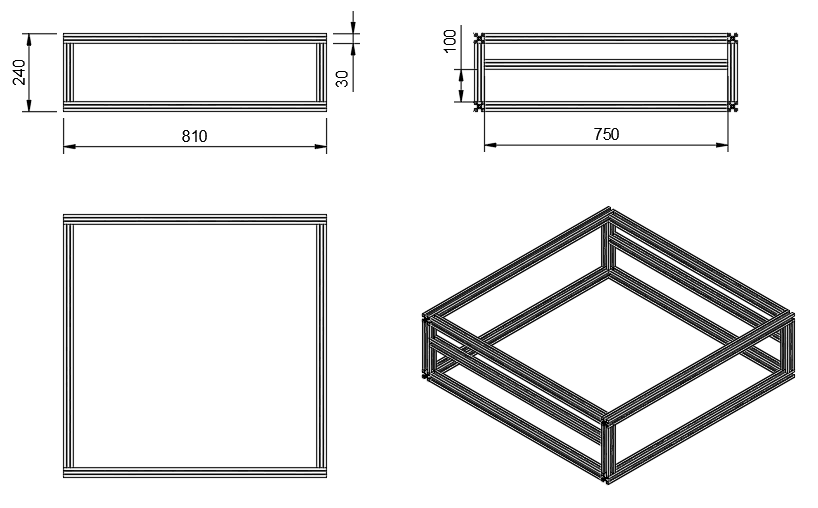
\includegraphics[width=0.8\textwidth]{PLANOS/PLANOS_CAJON_INTERNO_1.png}
            \caption{Plano del cajón interno de la Estación de Carga}
            \label{fig:etiqueta}
        \end{figure}
        
 Por consiguiente, tomando en cuenta las dimensiones del plano anterior, se realizó lo que es el "cajón externo" en el cual sirve para almacenar el dron y la electrónica de la estación de carga. Esto se puede observar en la Fig 2.
        \begin{figure}[htpb]
            \centering
            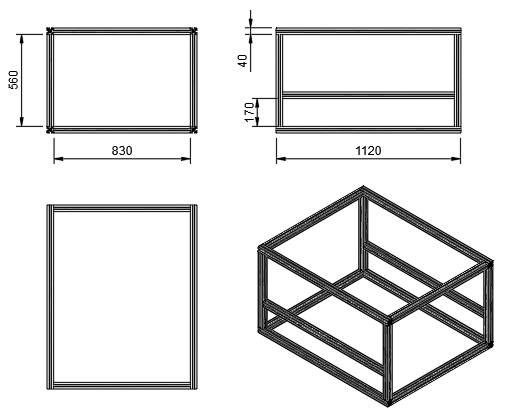
\includegraphics[width=0.8\textwidth]{PLANOS/PLANOS_CAJON_EXTERNO_1.png}
            \caption{Plano del cajón externo de la Estación de Carga}
            \label{fig:etiqueta}
        \end{figure}

Después, se tomaron en cuenta las dimensiones de las landing gear (patas del dron) para imprimir en 3D unas guías mecánicas (Fig 3.) que ayuden a estas mismas a hacer una correcta conexión magnética con el sistema de carga.
        \begin{figure}[htpb]
            \centering
            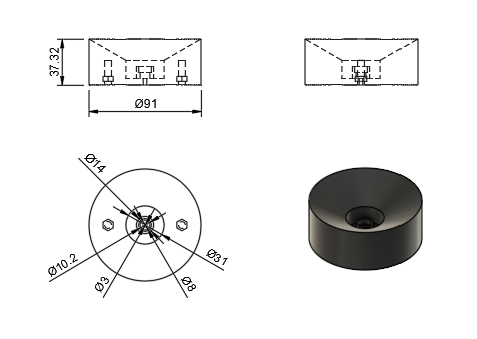
\includegraphics[width=0.8\textwidth]{PLANOS/PLANO_GUIAS_MECANICAS.png}
            \caption{Plano de guía mecánica para la Estación de Carga}
            \label{fig:etiqueta}
        \end{figure}

Tomando en cuenta los diseños de la Fig. 1 y la Fig. 3 se desarrolló por completo el diseño de el cajón interno (Fig. 4), cuenta con dos cortes de MDF de 9 mm de 810 mm x 810 mm y separadores internos con espacio de 20 mm de altura para proteger los cables del sistema de carga. 

        \begin{figure}[htpb]
            \centering
            %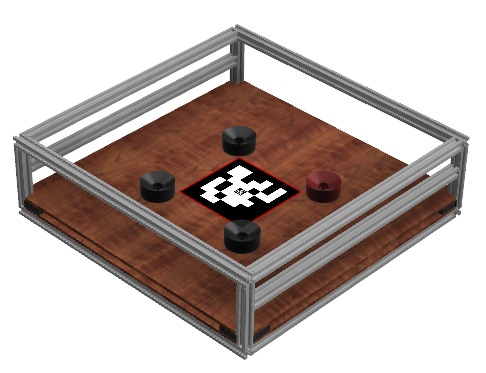
\includegraphics[width=0.6\textwidth]{PLANOS/CAJON_INTERNO_FINAL.png}
            \caption{Vista del cajón interno de la Estación de Carga.}
            \label{fig:etiqueta}
        \end{figure}


Se desarrollaron los diseños CAD necesarios como se muestran en la Fig 5. y Fig 6. para garantizar la correcta integración y adaptación de los distintos componentes de la estación de carga. Estos diseños permitieron establecer las dimensiones, tolerancias y características esenciales para que cada elemento se ajustara de manera precisa, asegurando que la estación de carga cumpliera con su funcionalidad de forma eficiente y confiable.

\begin{figure}[h]
    \centering
    \begin{minipage}{0.45\textwidth}
        \centering
        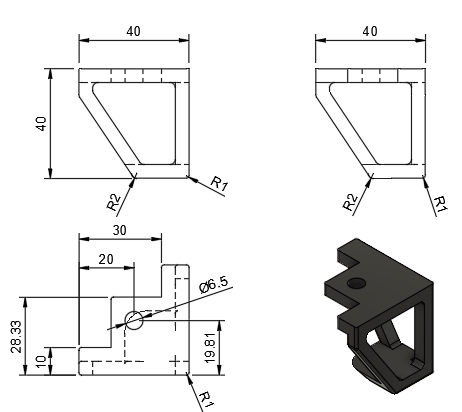
\includegraphics[width=\textwidth]{PLANOS/PLANO_PATAS_ESTABILIDAD_CAJON.png}
        \caption{Soportes de piso para la estabilidad de la Estación de Carga.}
        \label{fig:imagen1}
    \end{minipage}%
    \hfill
    \begin{minipage}{0.45\textwidth}
        \centering
        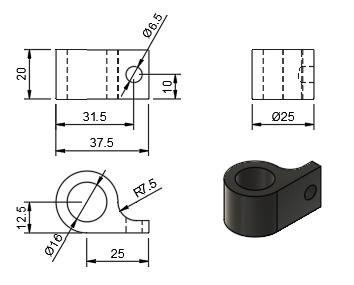
\includegraphics[width=\textwidth]{PLANOS/PLANO_SENSOR.png}
        \caption{Sujetador impreso en 3D para los sensores de proximidad inductivos de la Estación de Carga.}
        \label{fig:imagen2}
    \end{minipage}%
    \hfill
\end{figure}

Por último del proceso de diseño, se desarrolló un modelo CAD que integra los componentes principales necesarios para el correcto funcionamiento de la estación de carga. Este diseño conceptual final, mostrado en la figura 7, representa la consolidación de las ideas iniciales, las iteraciones realizadas y las decisiones tomadas a lo largo del desarrollo. El modelo asegura la funcionalidad, compatibilidad y eficiencia de la estación, sirviendo como base para la fabricación e implementación del sistema.

        \begin{figure}[htpb]
            \centering
            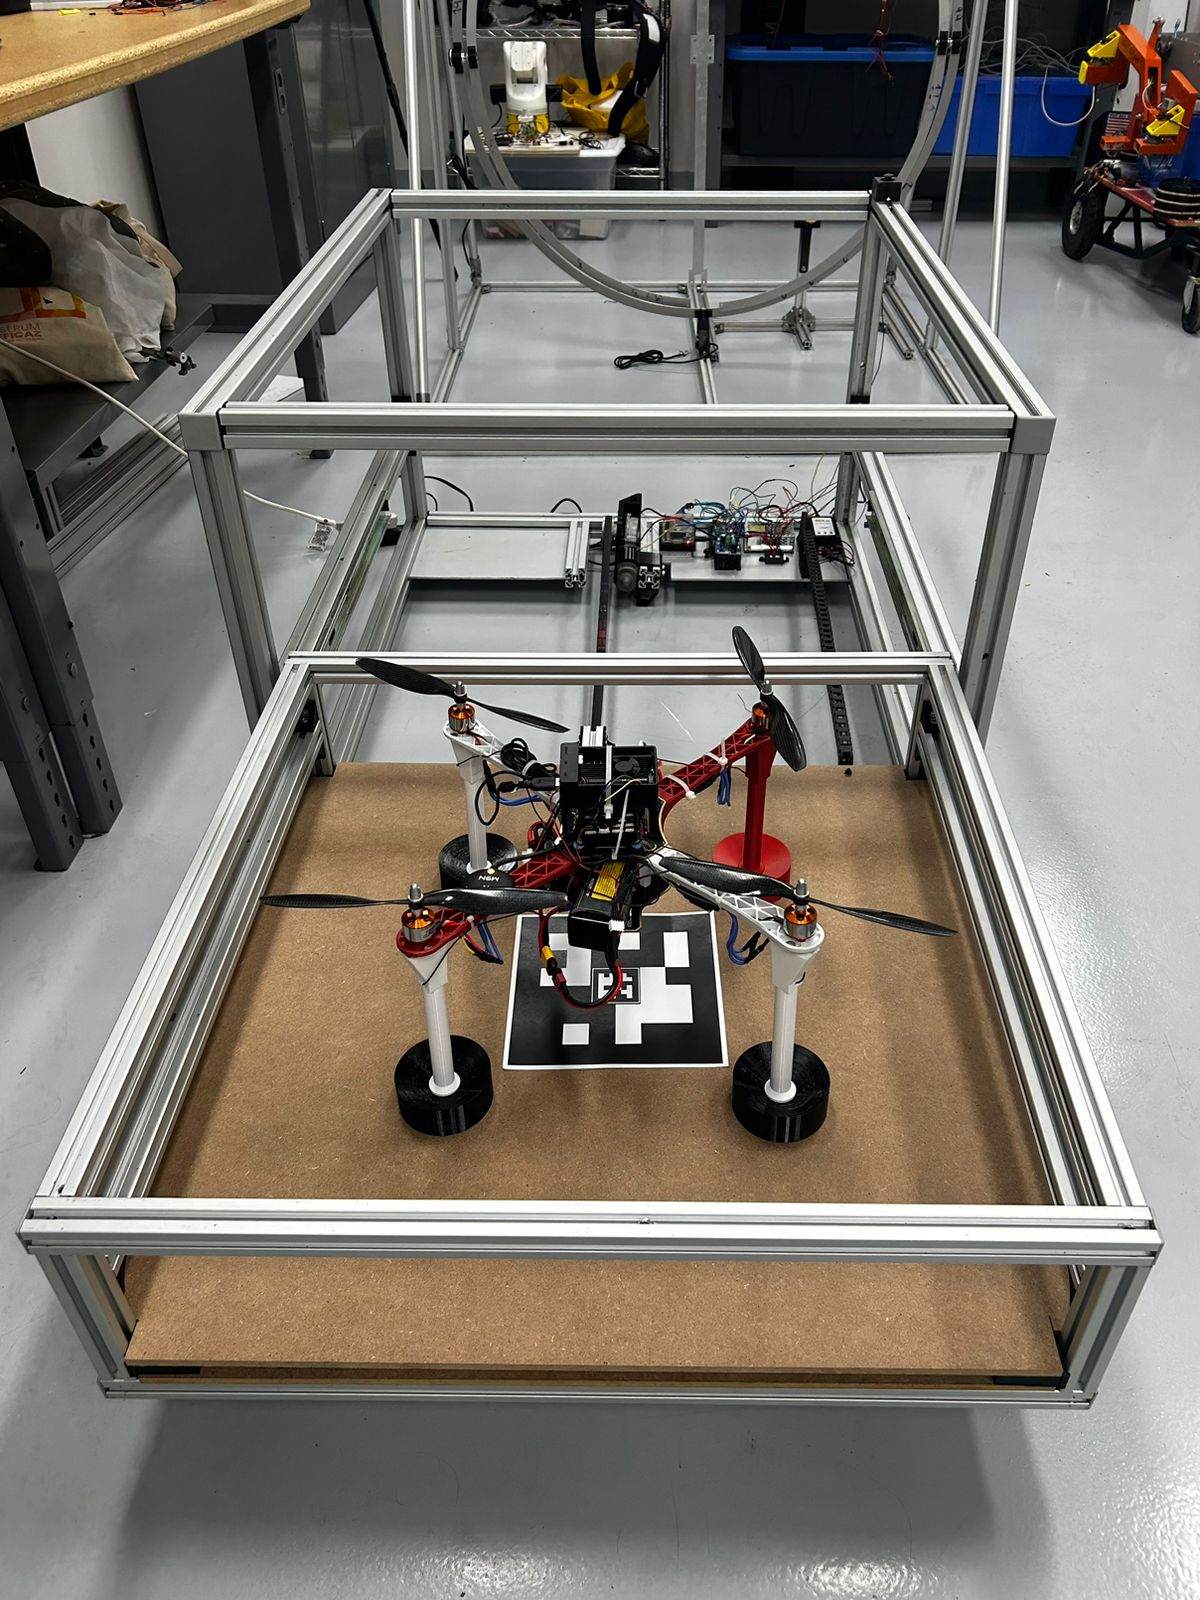
\includegraphics[width=1\textwidth]{pictures/ESTACION_FINAL.jpg}
            \caption{Vista de la Estación de Carga.}
            \label{fig:etiqueta}
        \end{figure}

\subsection{Selección e Implementación del Mecanismo de Movimiento del Cajón}

El diseño del mecanismo de cajón automático para la estación de carga pasó por varias etapas de conceptualización, considerando diferentes opciones para garantizar un movimiento eficiente y económico. Inicialmente, se planteó utilizar una banda dentada similar al mecanismo de las impresoras 3D, permitiendo un desplazamiento preciso hacia adelante y hacia atrás; sin embargo, esta solución resultaba costosa y compleja debido a las dimensiones requeridas. Como alternativa, se evaluó el uso de pistones, pero estos incrementaban aún más los costos del proyecto. Finalmente, se optó por implementar un sistema de banda y polea tipo V, clasificación A, debido a su rápida disponibilidad y considerable reducción en costos, logrando así un equilibrio entre funcionalidad, simplicidad y economía.

\subsubsection{Componentes y Diseños CAD}
    \begin{enumerate}
        \item Motor de 12V
            \begin{figure}[htpb]
                \centering
                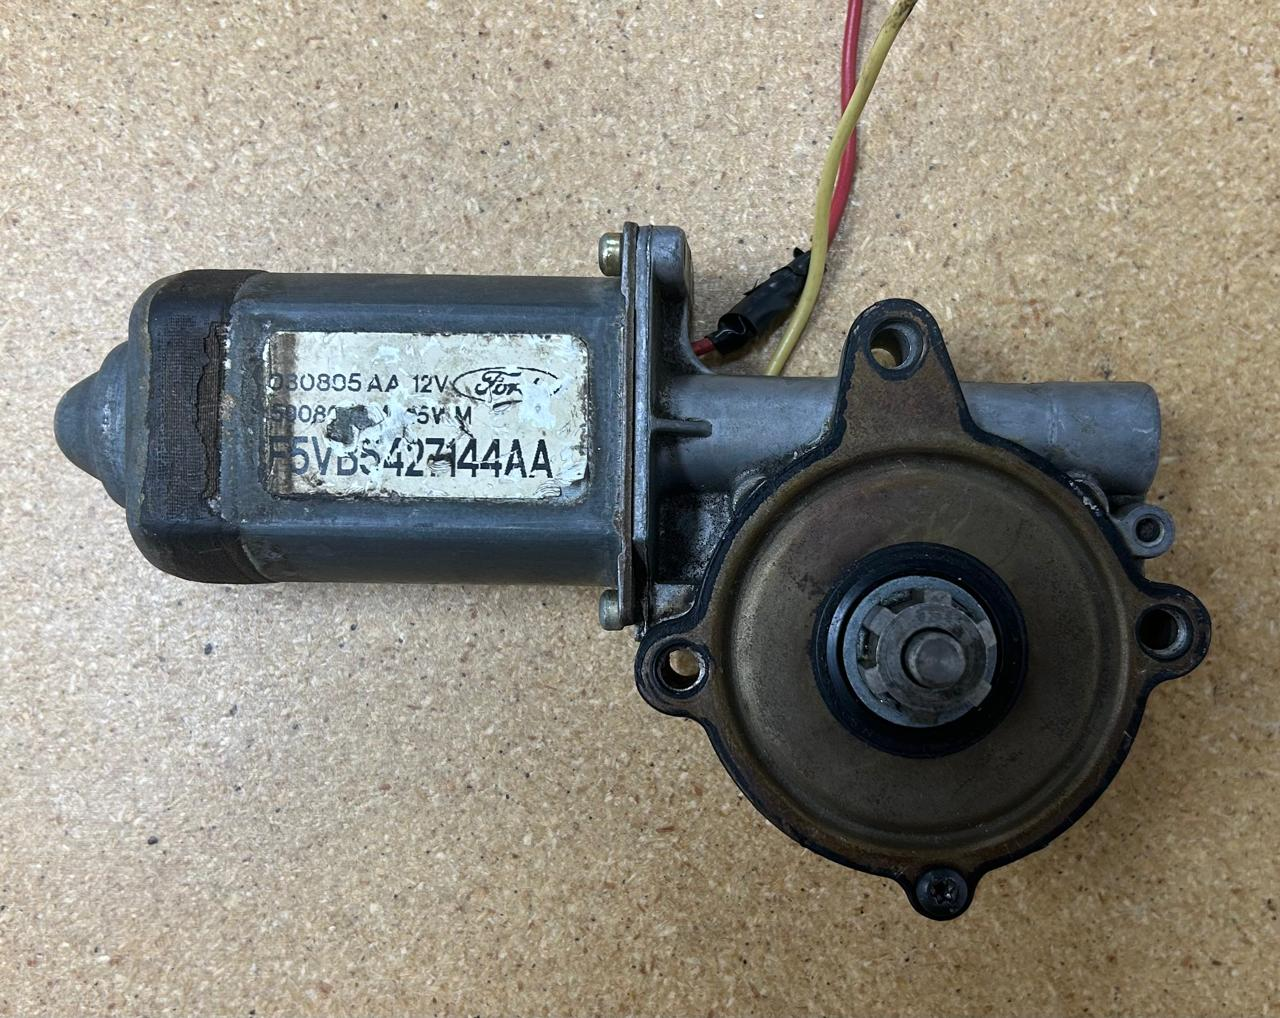
\includegraphics[width=0.4\textwidth]{MECANISMO/MOTOR_12V.jpg}
                \caption{Motor de 12 Volts utilizado para la Estación de Carga.}
                \label{fig:etiqueta}
            \end{figure}
        \item Poleas
            \begin{figure}[htpb]
                \centering
                %\includegraphics[width=0.35\textwidth]{MECANISMO/POLEA_ALUMINIO-removebg-preview.png}
                \caption{Polea de aluminio con diametro interno de 1/2"}
                \label{fig:etiqueta}
            \end{figure}
        \item Banda V Tipo A
        \begin{figure}[htpb]
                \centering
                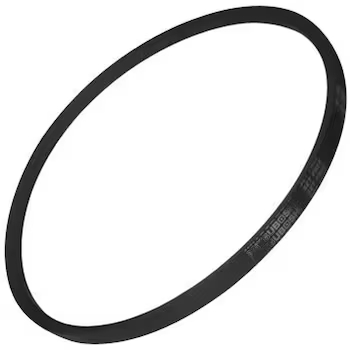
\includegraphics[width=0.35\textwidth]{MECANISMO/BANDA_V_TIPOA-transformed.jpg}
                \caption{V-Belt Type }
                \label{fig:etiqueta}
            \end{figure}
        \item Baleros
        \begin{figure}[htpb]
                \centering
                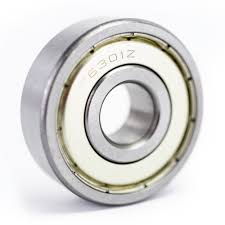
\includegraphics[width=0.35\textwidth]{MECANISMO/balero.jpeg}
                \caption{Baleros de..}
                \label{fig:etiqueta}
            \end{figure}
        \item Chumaceras 
        \begin{figure}[htpb]
                \centering
                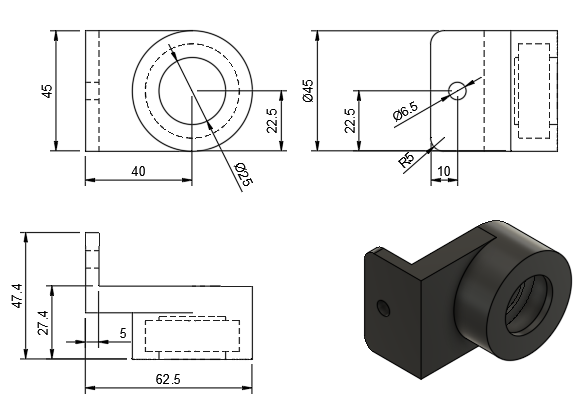
\includegraphics[width=0.35\textwidth]{PLANOS/PLANO_CHUMACERA.png}
                \caption{Plano de chumaceras para el mecanismo de movimiento del cajón interno.}
                \label{fig:etiqueta}
            \end{figure}
        \item Sujetadores de Motor 12 V
            \begin{figure}[h]
            \centering
            \begin{minipage}{0.45\textwidth}
                \centering
                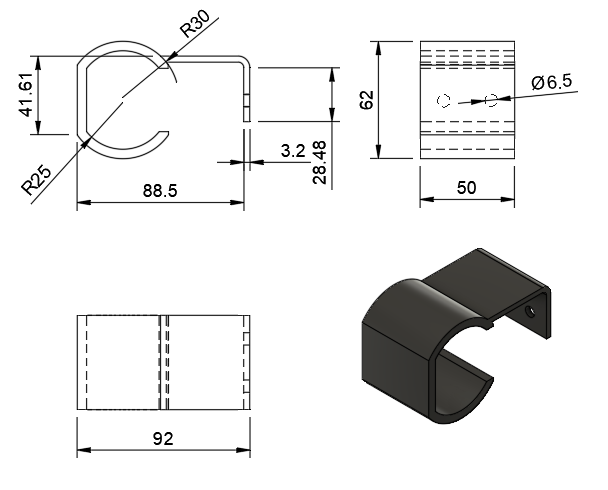
\includegraphics[width=\textwidth]{PLANOS/PLANO_SOPORTE_MOTOR_1.png}
                \caption{}
                \label{fig:imagen1}
            \end{minipage}%
            \hfill
            \begin{minipage}{0.45\textwidth}
                \centering
                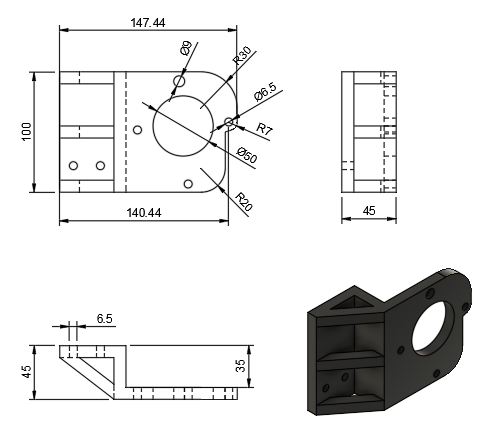
\includegraphics[width=\textwidth]{PLANOS/PLANO_SOPORTE_MOTOR_2.png}
                \caption{}
                \label{fig:imagen2}
            \end{minipage}%
            \hfill
            \end{figure}
        \item Sujetador de Banda V para cajón interno.
            \begin{figure}[h]
            \centering
            \begin{minipage}{0.45\textwidth}
                \centering
                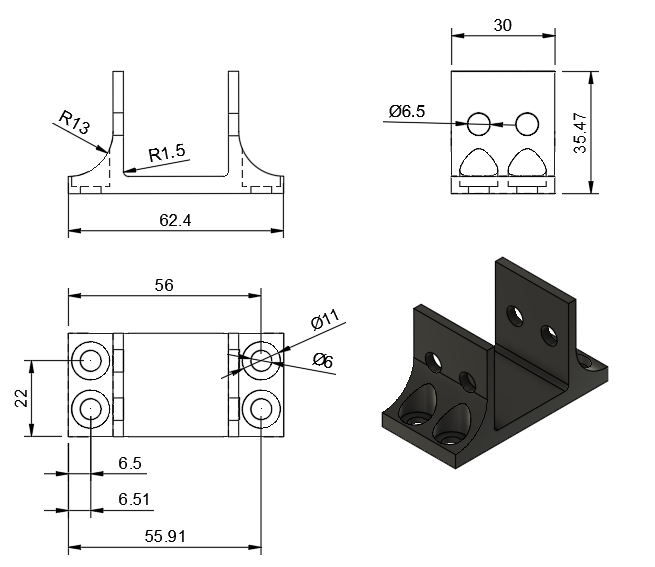
\includegraphics[width=\textwidth]{PLANOS/PLANO_SUJ_BANDA_1.png}
                \caption{}
                \label{fig:imagen1}
            \end{minipage}%
            \hfill
            \begin{minipage}{0.45\textwidth}
                \centering
                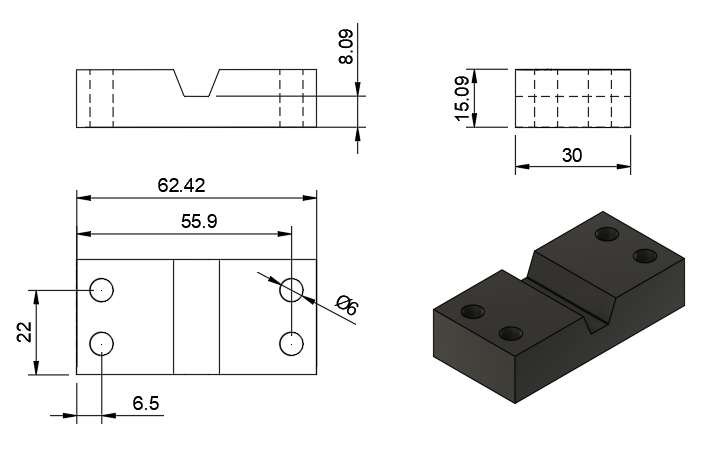
\includegraphics[width=\textwidth]{PLANOS/PLANO_SUJ_BANDA_2.png}
                \caption{}
                \label{fig:imagen2}
            \end{minipage}%
            \hfill
            \end{figure}
    \end{enumerate}

\subsubsection{Mecanismo Polea y Banda tipo V}

\begin{figure}[h]
    \centering
    \begin{minipage}{0.49\textwidth}
        \centering
        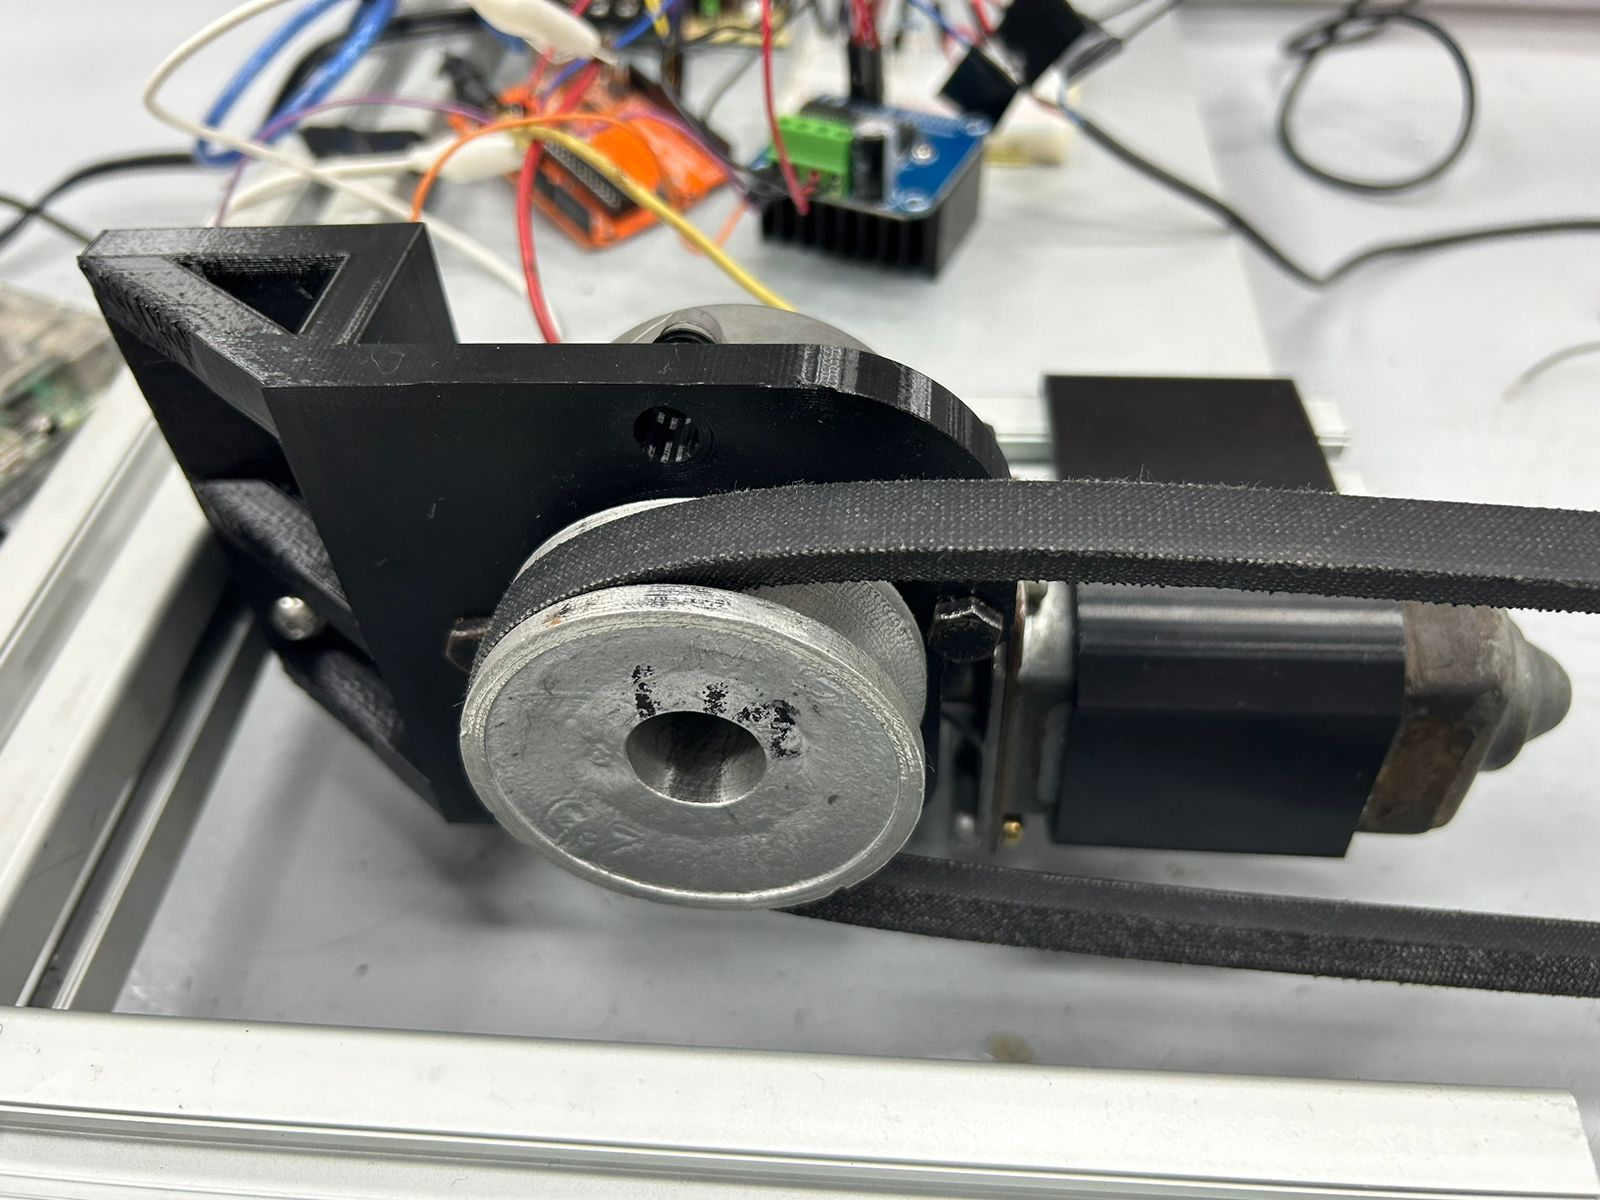
\includegraphics[width=\textwidth]{MECANISMO/MOTOR_MECANISMO.jpg}
        \caption{Vista del mecanismo para el movimiento del cajón interno, donde se muestran los sujetadores del motor impresos en 3D y el motor con la polea y la banda integradas al sistema.}
        \label{fig:imagen1}
    \end{minipage}%
    \hfill
    \begin{minipage}{0.49\textwidth}
        \centering
        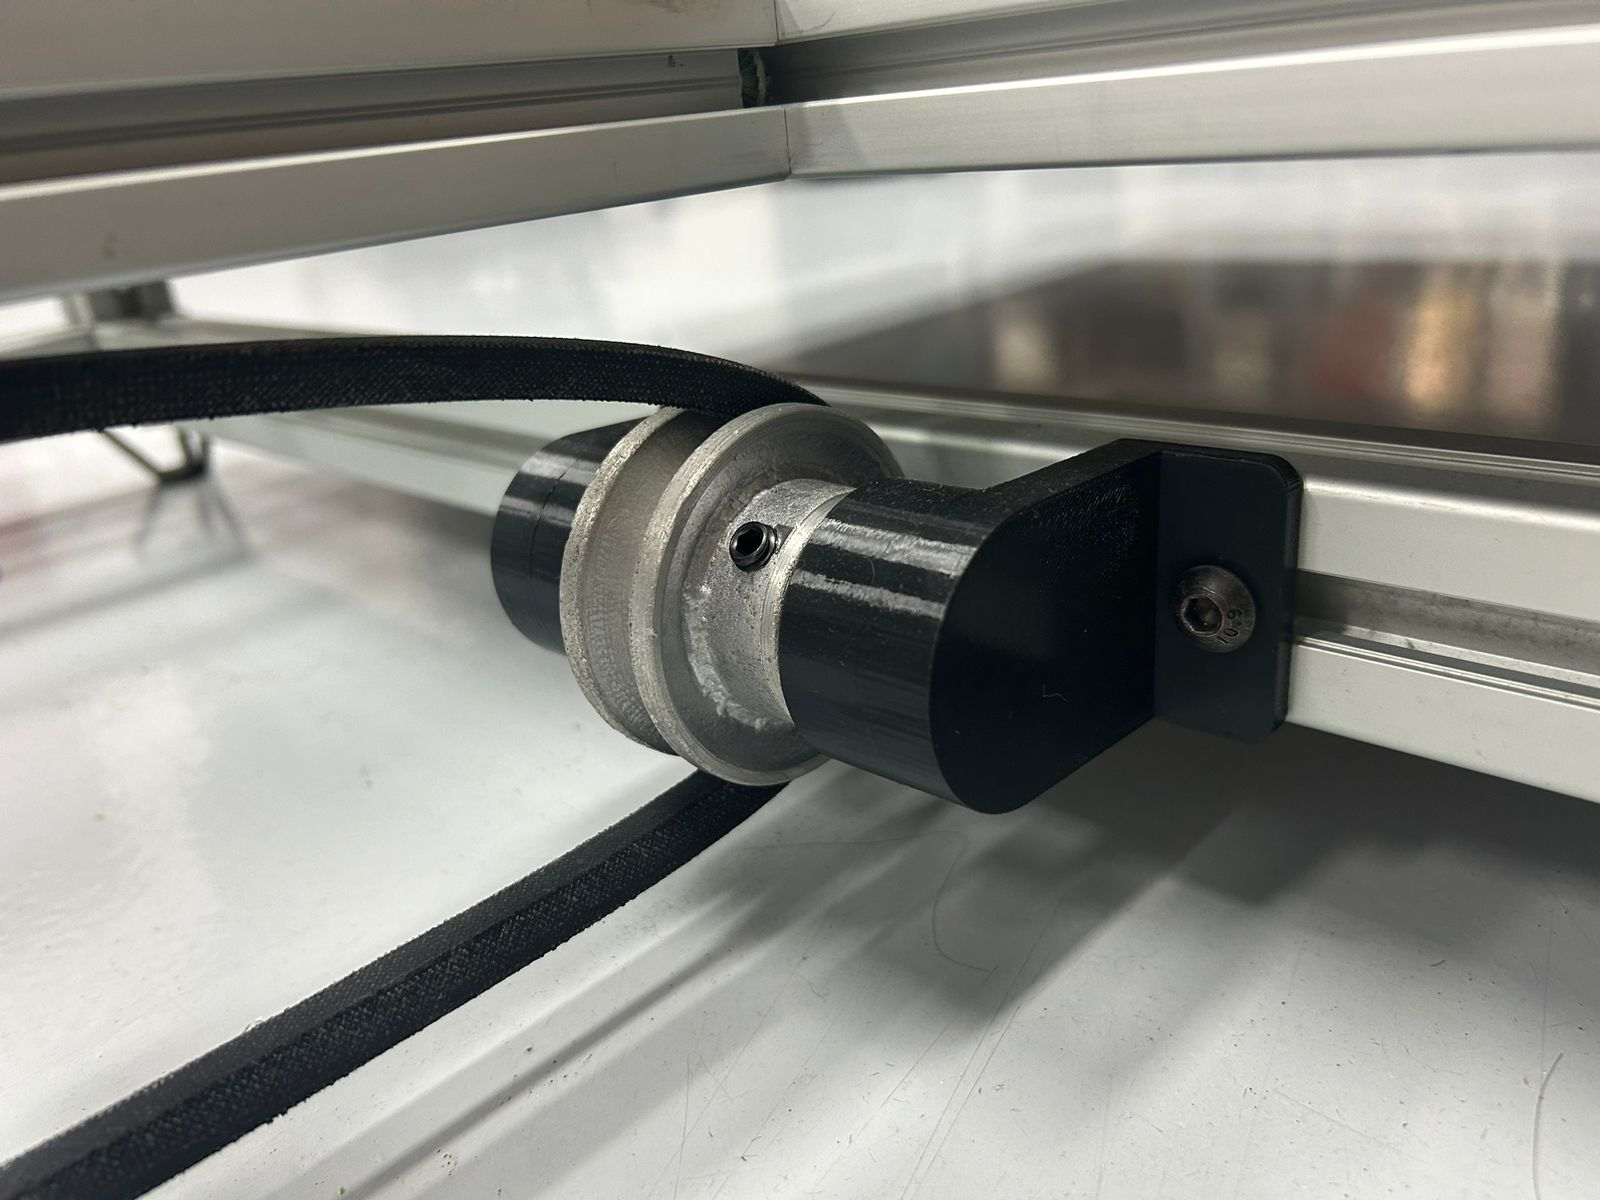
\includegraphics[width=\textwidth]{MECANISMO/MECANISMO_CHUMACERAS.jpg}
        \caption{Vista del mecanismo para el movimiento del cajón interno, donde se muestran las chumaceras impresas en 3D, con...}
        \label{fig:imagen2}
    \end{minipage}%
    \hfill
    \begin{minipage}{0.49\textwidth}
        \centering
        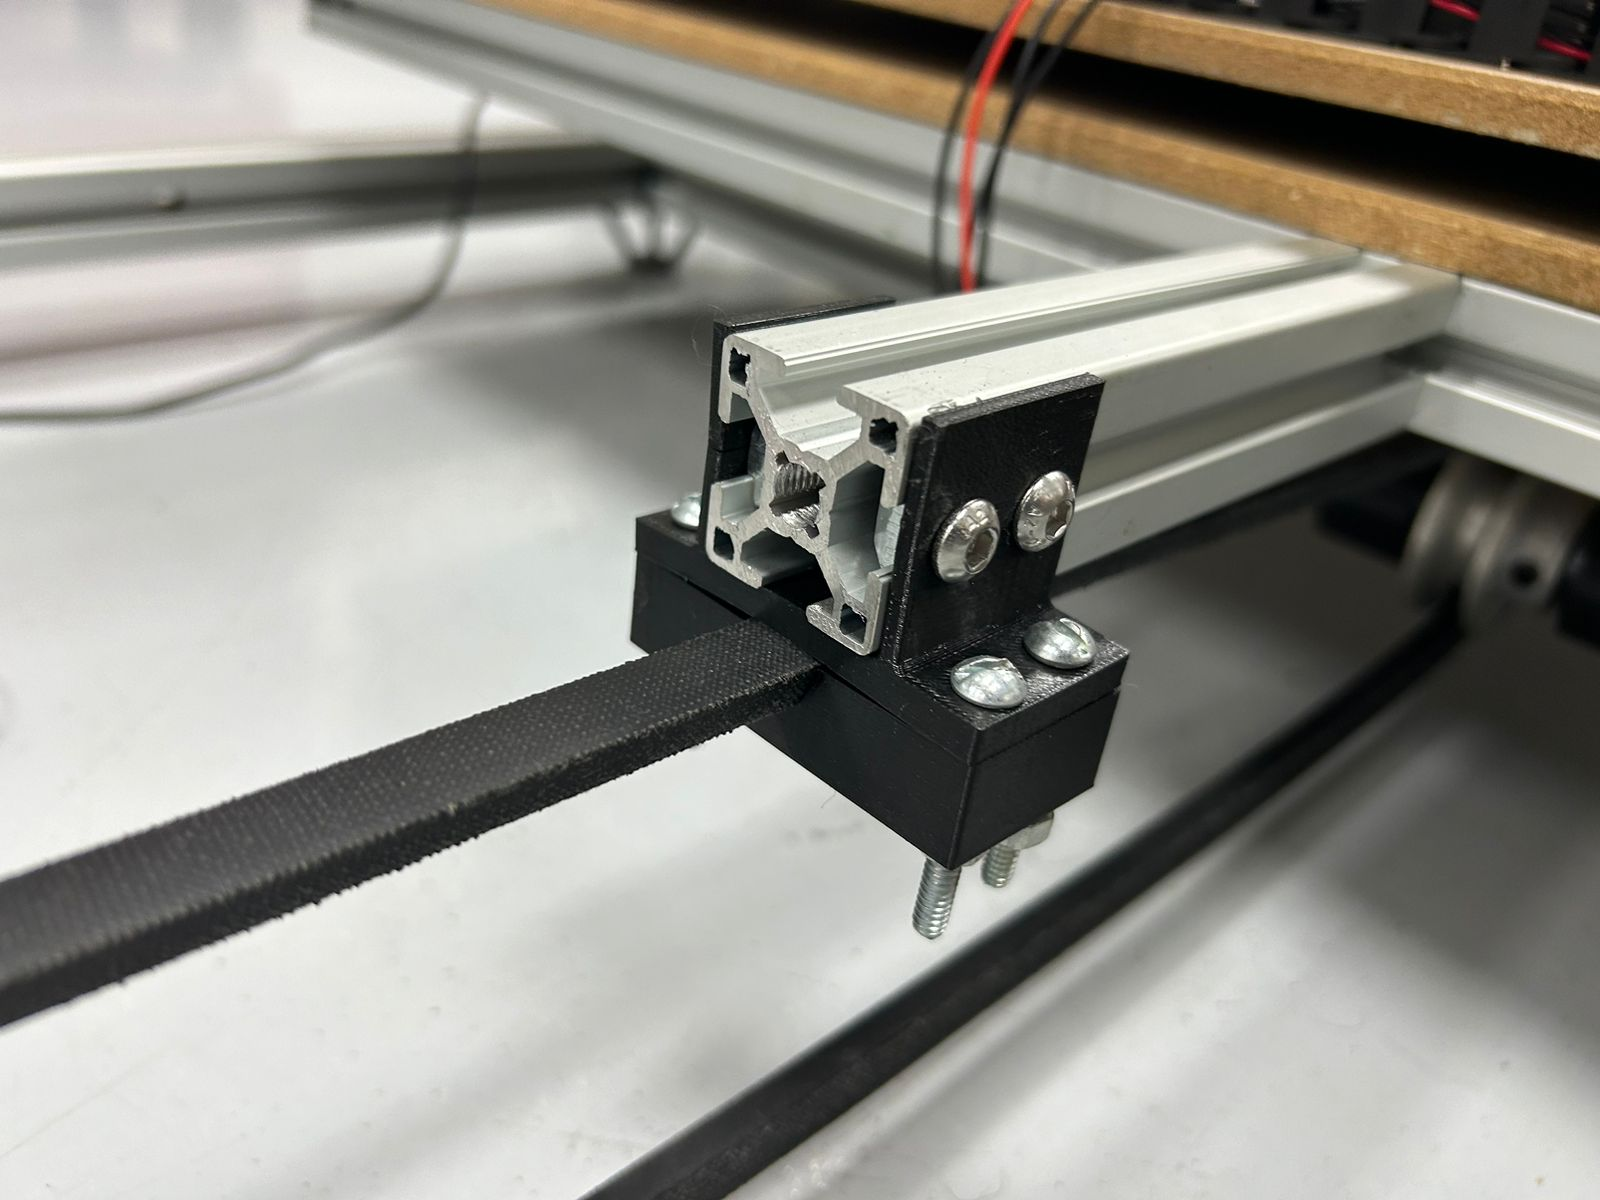
\includegraphics[width=\textwidth]{MECANISMO/MECANISMO_AGARRE.jpg}
        \caption{Vista del mecanismo para el movimiento del cajón interno, donde se muestran la sujeción que se imprimió en 3D para abrazar la banda con el cajón interno.}
        \label{fig:imagen1}
    \end{minipage}%
    \hfill
\end{figure}

\begin{figure}[htpb]
    \centering
    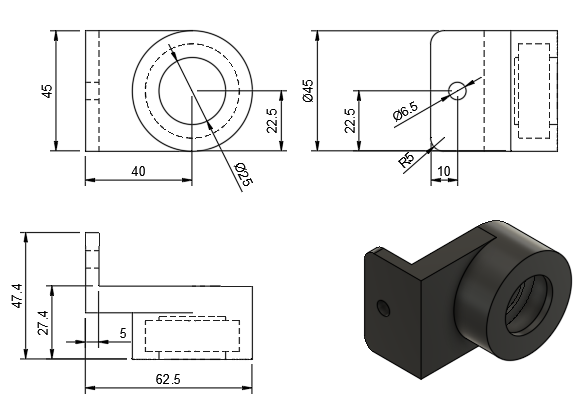
\includegraphics[width=0.35\textwidth]{PLANOS/PLANO_CHUMACERA.png}
    \caption{Plano de chumaceras para el mecanismo de movimiento del cajón interno.}
    \label{fig:etiqueta}
\end{figure}


\subsection{Proceso de Manufactura de la Estructura de la Base de Carga}

    \begin{enumerate}
        \item \textbf{Corte del Material:} Para iniciar el proceso de manufactura, se realizaron cortes precisos de los perfiles de aluminio y las placas de MDF según las dimensiones especificadas en la lista de materiales. Este paso es fundamental para asegurar que todas las piezas se ensamblen correctamente en el diseño modular. Se puede observar este preoceso en la Figura ? a) 
            
        \item \textbf{Ensamblaje de la Estructura:} Una vez cortadas las piezas, se procedió a ensamblar la estructura principal de la estación de carga utilizando tornillos y tuercas para fijar los perfiles de aluminio y las placas de MDF usando separadores de 20 mm impresos en 3D. Se verificó que todas las piezas estuvieran alineadas y niveladas para garantizar la estabilidad y resistencia de la base de carga. Esto se muestra en las Figura ? b) y c).
            
        \item \textbf{Instalación del Mecanismo de Movimiento:} Después de ensamblar la estructura principal, se instaló el mecanismo de polea y banda tipo V para permitir el movimiento horizontal del cajón. Se colocaron las poleas, la banda y el motor en las ubicaciones previamente definidas, asegurando que el sistema de movimiento funcionara correctamente y sin obstrucciones. Figura ? d).
        
    \end{enumerate}

    \begin{figure}[h!]
        \centering
        \begin{subfigure}[b]{0.4\textwidth}
            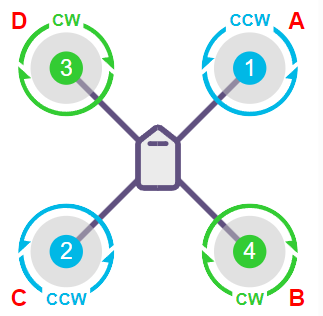
\includegraphics[width=\textwidth]{pictures/quad_frame.png}
            \caption{Quad X Frame.}
            \label{fig:quad_frame}
        \end{subfigure}
        \hfill
        \begin{subfigure}[b]{0.4\textwidth}
            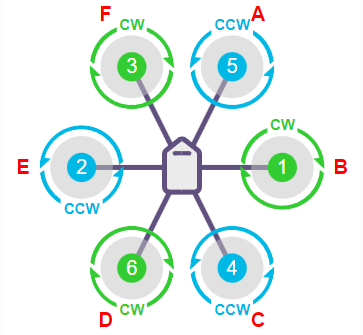
\includegraphics[width=\textwidth]{pictures/hexa_frame.png}
            \caption{Hexa X Frame.}
            \label{fig:hexa_frame}
        \end{subfigure}
        \vskip\baselineskip
        \begin{subfigure}[b]{0.4\textwidth}
            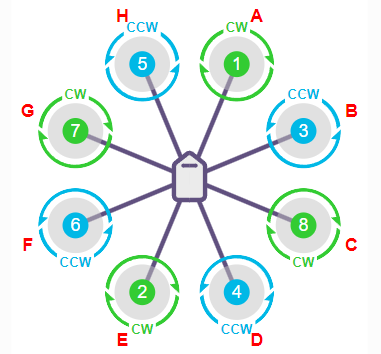
\includegraphics[width=\textwidth]{pictures/octo_frame.png}
            \caption{Octo X Frame.}
            \label{fig:octo_frame}
        \end{subfigure}
        \hfill
        \begin{subfigure}[b]{0.4\textwidth}
            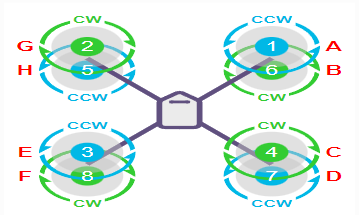
\includegraphics[width=\textwidth]{pictures/octo_quad_frame.png}
            \caption{Octo Quad X Frame.}
            \label{fig:octo_quad_frame}
        \end{subfigure}
        \caption{Drone configurations.}
        \label{fig:drone_frames}
    \end{figure}

%%ANABI starts

    \subsection{Electronic Circuit of the Charging Station}

    \subsubsection{Conection Diagram}
    add diagram circuit
    
    \subsubsection{Circuit Construction}
    add images
    
    \subsubsection{Circuit Programming}
    
    \paragraph{\textbf{General Description:}}
    
    
    The described circuit uses a joystick to control a motor that moves a drawer back and forth. The joystick is connected to a microcontroller (Arduino Mega 2560), which reads the joystick's Y-axis values to determine the direction in which the motor should move. Depending on the position of the joystick, the motor moves forward, backward or stops. In addition, limit switches are used to ensure that the motor stops when the drawer reaches its extreme positions.
    
    
    
    \paragraph{\textbf{Main Components}
    }
    \begin{itemize}
        \item \textbf{Arduino:} Microcontroller that manages the reading of the joystick values and controls the motor.
        \item \textbf{Joystick:} Analog input device that allows the user to control the direction of movement.
        \item \textbf{Motor and H-Bridge:} Driver system that moves the drawer. The H-bridge allows controlling the direction and speed of motion of the motor.
        \item \textbf{Limit Switches:} Sensors that detect when the drawer has reached its extreme positions (forward and reverse).
        \item \textbf{Power Supply:} Supplies power to the motor. The Arduino and RaspberryPi4 are supplied power by a plug-in charger.
    \end{itemize}
    
    
    \paragraph{\textbf{Arduino Code}
    }
    
    The Arduino code performs the following functions:
    
    \begin{enumerate}
        \item \textbf{Pin initialization:}
        \begin{itemize}
            \item The joystick pins (A1 for the Y-axis) are configured as inputs.
            \item Motor pins 9 and 8 are configured as outputs.
            \item The limit switch pins (10 and 11) are configured as inputs with internal pull-up resistors.
        \end{itemize}
        \item \textbf{Reading of Joystick:}
        \begin{itemize}
            \item At each loop cycle, the Arduino reads the analog value from the joystick's Y-axis.
            \item Depending on the value read, the Arduino decides whether the motor should move forward, backward or stop.
        \end{itemize}
        \item \textbf{Motor Control:}
        \begin{itemize}
            \item If the value of the joystick Y-axis is greater than 512 (middle position) and the forward limit switch is not pressed, the motor moves forward.
            \item If the Y-axis value is less than 512 and the backward limit switch is not pressed, the motor moves backward.
            \item If the Y-axis value is approximately 512 or any limit switch is pressed, the motor stops.
        \end{itemize}
        \item \textbf{Limit Switch Verification:}
        \begin{itemize}
            \item If the motor is moving forward and the forward limit detects  metal (the drawer), the motor stops.
            \item If the motor is moving backward and the backward limit switch detects  metal (the drawer), the motor stops.
    
        \end{itemize}
        
    \end{enumerate}
    
    %%%%%CODIGOOOOOOOO (??????)
    
    \paragraph{\textbf{Circuit Operation}
    }
    \begin{itemize}
        \item Initialization: At startup, the Arduino configures the pins and establishes serial communication for debugging.
    \item Continuous Readout: In the main loop, the Arduino continuously reads the value of the joystick Y-axis.
    \item Dynamic Control: Based on the value read, the Arduino controls the motor to move the drawer forward, backward or stop it.
    \item Safety Check: Limit switches ensure that the motor automatically stops when the drawer reaches its extreme positions, protecting the system from possible damage.
    \item Debugging: Joystick values and motor status are printed on the serial monitor for easy debugging and system tuning.
    \end{itemize}
    
    \paragraph{\textbf{Annex}
    }
    %\paragraph{
    The complete source code for both the Arduino and Raspberry Pi 4 is included in the appendices of this document, making it easy to review and modify as needed for implementation and control of the system.
    
    This approach ensures that the drawer moves in a precise and controlled manner based on the joystick position, providing an efficient solution for linear motion control using a motor and belt.

%%ANABI ENDS
    







\section{Drone Instrumentation}

\subsection{Specifications and Requirements}
To ensure compatibility and functionality in the charging system, the drone must meet the following specifications:
    \begin{itemize}
        \item The dimensions of the parts must be adapted to the frame of the quadcopter drone of open architecture that was purchased.
        \item The drone must have a charging circuit compatible with the charging station.
        \item The drone must have a camera and a vision system for the detection of ArUco markers.
        \item Location sensors shall be integrated for outdoor navigation.
        \item A microprocessor should be integrated as an auxiliary computer for data processing and communication with the charging station.
    \end{itemize}

\subsection{Drone Instrumentation Materials List} 
    \begin{itemize} 
        \item 1 x Open quadcopter frame (F450) 
        \item 1 x Flight Controller (PIxHawk 6x) 
        \item 1 x Camera (compatible with ArUco detection) 
        \item 1 x Raspberry Pi 4 (Companion Computer) 
        \item 1 x Proximity Sensor (model of preference) 
        \item 1 x GPS Module (compatible with flight controller) 
        \item Wiring and connectors 
        \item 3D printed mounting hardware (specific brackets for each component) 
    \end{itemize}

\subsection{Drone CAD drawings} 
Presented below are the CAD designs of the parts that have been developed for the drone, adapted to its original frame to integrate the necessary electronic components and meet the loading and positioning requirements.
    \begin{itemize} 
        \item New brackets were designed for the microprocessor and camera, ensuring stable and precise integration into the frame. 
        \item A mounting space for the location sensors and charging circuitry was implemented. 
        \begin{center} 
            \textit{Image of the CAD designs of the drone with the modified parts.} 
        \end{center} 
    \end{itemize}

    \subsection{Power Distribution Circuit} 
    The power distribution circuit was designed to provide safe and stable power to the drone's critical components, including the motors, flight controller, Raspberry Pi 5, and camera. The operation of each section of the circuit is described below:
    
    \begin{enumerate}
        \item \textbf{3S LiPo battery:} 
        A 3-cell lithium-polymer (LiPo) battery with a capacity of 5200 mAh, a nominal voltage of 11.1 V and a discharge rate of 50 C was selected. This battery is ideal for providing the necessary current for the motors and electronics without compromising flight duration.

        \item \textbf{Power distribution to the motors:} 
        Power from the battery is distributed through a power distribution board, which connects the battery to the four electronic speed controllers (ESCs). Each ESC regulates the power sent to its respective A2212 10T motor, allowing precise speed control of the motors.
    
        \item \textbf{Voltage regulator XL4005 DC-DC:} 
        This regulator converts the 11.1 V battery voltage to 5 V, providing stable and safe power supply for the Raspberry Pi and the connected camera.
    
        \item \textbf{Flight controller Pixhawk 6X RT:} 
        The flight controller is connected directly to the power distribution board to receive the necessary power. It also manages communication with the ESCs and other sensors on the drone, such as the GPS module (M9N) connected to the GPS1 port.

        \item \textbf{Raspberry Pi 5:} 
        The Raspberry Pi is powered through the voltage regulator and connects to the flight controller via a serial port to receive data and send commands to the system. It also manages the USB-connected camera, which captures images for real-time processing.
    
        \item \textbf{GPS Module M9N:} 
        This module connects to the Pixhawk controller via the GPS1 port to provide real-time outdoor positioning data essential for drone navigation.
    
    \end{enumerate}
    
    \begin{center}
        \begin{figure}[h!]
            \centering
            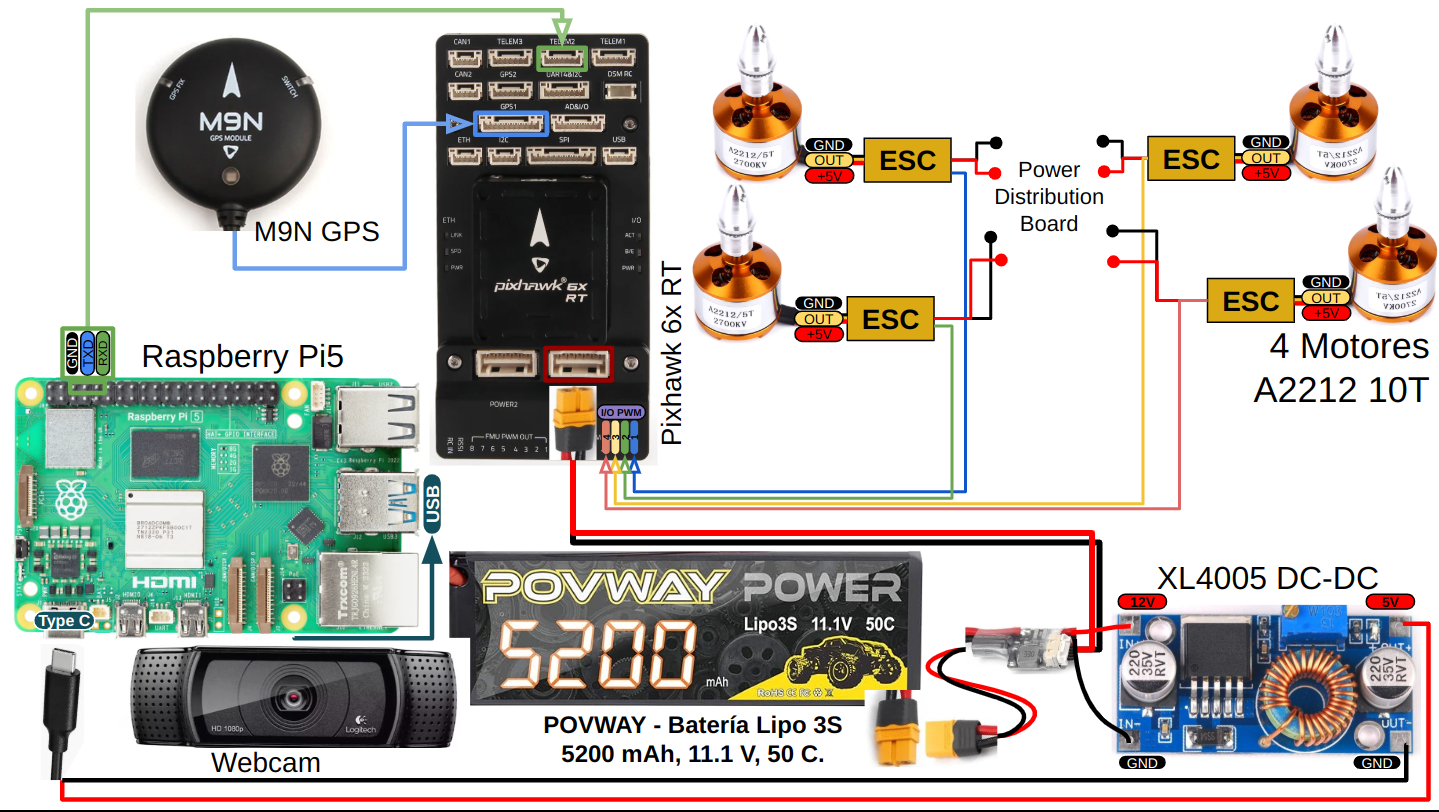
\includegraphics[width=0.8\textwidth]{pictures/drone_electronic_diagram.png}
            \caption{Diagram of the power distribution circuit of the drone}.
        \end{figure}
    \end{center}
        

\section{Software Configuration}

\subsection{Ground Host Computer Configuration} 
The central computer was configured to monitor and process the information coming from the drone's auxiliary computer. The steps performed for this configuration are described below:
\begin{itemize}
    \item \textbf{Installation of ROS 2 Humble:} 
    Since the host computer is running Ubuntu 22.04, ROS 2 Humble was installed following the official instructions. The commands used were:    \begin{verbatim}
    sudo apt update && sudo apt install -y software-properties-common
    sudo add-apt-repository universe
    sudo apt update
    sudo apt install -y ros-humble-desktop
    \end{verbatim}
    This included the installation of the necessary tools to develop and run applications on ROS 2 Humble.

    \item \textbf{Configuración del entorno:} 
    To facilitate the use of ROS 2, the file \texttt{~/.bashrc} was configured. The following line was added to the end of the file:
        \begin{verbatim}
    source /opt/ros/humble/setup.bash
    \end{verbatim}
    It was subsequently executed:
    \begin{verbatim}
    source ~/.bashrc
    \end{verbatim}

    \item \textbf{GitHub repository cloning:} 
    A workspace was created for ROS 2 and the corresponding repository was cloned. The steps performed were:
    \begin{verbatim}
    mkdir -p ~/ros2_ws/src
    cd ~/ros2_ws/src
    git clone <URL_del_repositorio>
    cd ..
    colcon build
    \end{verbatim}

    \item \textbf{\texttt{ROS\_DOMAIN\_ID} Configuration:} 
    To ensure proper communication between the host computer and the drone's auxiliary computer, the \texttt{ROSAIN_ID} was configured with the value 10. This was done by adding the following line to the \texttt{~/.bashrc} file:    \begin{verbatim}
    export ROS_DOMAIN_ID=10
    \end{verbatim}
    It was then executed:    \begin{verbatim}
    source ~/.bashrc
    \end{verbatim}
    
    \item \textbf{ROS 2 environment Verification:} 
    Finally, the environment was verified to be correctly configured using the following commands:
    \begin{verbatim}
    ros2 doctor
    \end{verbatim}
    This allowed us to confirm that all the necessary dependencies for ROS 2 Humble were installed and working correctly.    
    \begin{center} 
        \textit{Image of the environment configuration on the main computer.} 
    \end{center}
\end{itemize}


\subsection{Configuration of the Drone Auxiliary Computer} 
The Raspberry Pi 5 was configured as an auxiliary computer for data processing and real-time communication with the charging station. The steps performed for its configuration are detailed below:

    \begin{itemize}
        \item \textbf{Installing Ubuntu 24.04:} 
        The Raspberry Pi Imager tool was used to install Ubuntu Server 24.04 LTS (64-Bit) on the SD card. During the initial setup, SSH was enabled, a user with password was defined and the Raspberry Pi was connected to the Wi-Fi network.
    
        \item \textbf{Initial connection and SSH:} 
        After inserting the SD card into the Raspberry Pi and connecting it to a monitor and keyboard, the device was powered on, and the configured credentials were entered. The IP address was obtained using the command:
        \begin{verbatim}
        hostname -I
        \end{verbatim}
        With this information, an SSH connection was established from an external computer using:        \begin{verbatim}
        ssh <usuario>@<IP>
        \end{verbatim}
        This allowed to continue with the configuration of the Raspberry Pi remotely.

        \item \textbf{System upgrade:} 
        A complete operating system upgrade was performed with the following commands:
        \begin{verbatim}
        sudo apt update && sudo apt upgrade -y
        \end{verbatim}
        \texttt{raspi-config} was also installed to enable the serial port. This option was configured in \texttt{Interface Options > Serial Port}, selecting \texttt{No} and then \texttt{Yes}.

        \item \textbf{Modification of \texttt{bashrc} and ID configuration:} 
        To ensure communication between all devices, the \texttt{ROSAIN_ID} was set to 10. The \texttt{~/.bashrc} file was edited with:        \begin{verbatim}
        sudo vim ~/.bashrc
        \end{verbatim}
        At the end of the file, the following lines were added:
                \begin{verbatim}
        export ROS_DOMAIN_ID=10
        source /opt/ros/jazzy/setup.bash
        \end{verbatim}
        Subsequently, the changes were saved and executed:
        \begin{verbatim}
        source ~/.bashrc
        \end{verbatim}
    
        \item \textbf{ROS 2 Jazzy Installation:} 
        Official instructions were followed to install ROS 2 Jazzy on Ubuntu 24.04. This included the commands:
                \begin{verbatim}
        sudo apt install -y software-properties-common
        sudo add-apt-repository universe
        sudo apt update
        sudo apt install -y ros-jazzy-desktop
        \end{verbatim}
    
        \item \textbf{GitHub repository cloning:} 
        A workspace was created in ROS 2 to integrate the custom nodes. The steps performed were:       
         \begin{verbatim}
        mkdir -p ~/ros2_ws/src
        cd ~/ros2_ws/src
        git clone <URL_del_repositorio>
        cd ..
        colcon build
        \end{verbatim}
    %%%anabi aqui
        \item \textbf{Instalación de MAVROS y MAVProxy:} 
        Para la comunicación con el Pixhawk, se instalaron MAVROS y MAVProxy. Los comandos utilizados fueron:
        \begin{verbatim}
        sudo apt install ros-jazzy-mavros ros-jazzy-mavros-extras
        sudo rosdep init
        rosdep update
        sudo apt install python3-mavproxy
        \end{verbatim}
        Además, se configuraron los complementos geográficos necesarios:
        \begin{verbatim}
        sudo apt install geographiclib-tools
        sudo geographiclib-get-geoids egm96-5
        \end{verbatim}
    
        \item \textbf{Verificación de la comunicación:} 
        Para garantizar que MAVROS y MAVProxy funcionaran correctamente, primero se inició MAVProxy con:
        \begin{verbatim}
        mavproxy.py --master=/dev/ttyAMA0 --baudrate 921600
        \end{verbatim}
        Posteriormente, se lanzó MAVROS utilizando:
        \begin{verbatim}
        ros2 launch mavros px4.launch fcu_url:=serial:///dev/ttyAMA0:921600
        \end{verbatim}
        Finalmente, se verificaron los tópicos disponibles con:
        \begin{verbatim}
        ros2 topic list
        \end{verbatim}
        y se confirmó la comunicación observando los mensajes de los tópicos relevantes.
        
        \begin{center} 
            \textit{Imagen de la configuración del entorno en la Raspberry Pi 5.} 
        \end{center}
    \end{itemize}
    
\subsection{Configuración de la Estación de Control en Tierra} 
    Se detalla la configuración realizada para la estación de control en tierra utilizando las herramientas QGroundControl y Mission Planner. Ambas aplicaciones son similares en funcionalidad, permitiendo la visualización y gestión de parámetros de vuelo. Sin embargo, dado que se utilizó ArduPilot como firmware, se decidió priorizar Mission Planner debido a su optimización para este sistema.
    
    \begin{itemize}
        \item \textbf{Instalación de Mission Planner y QGroundControl:} 
        Se instalaron ambas herramientas en la computadora central para la gestión y monitoreo del Pixhawk. Mission Planner se utilizó principalmente por su compatibilidad directa con ArduPilot, mientras que QGroundControl fue útil en ciertas configuraciones iniciales como algunas calibraciones redundates.
    
        \item \textbf{Calibración de sensores:} 
        La calibración de los sensores del Pixhawk que se realizó desde Mission Planner, siguiendo estos pasos:
        \begin{itemize}
            \item Acceder a la sección de calibración en la pestaña \textit{Initial Setup}.
            \item Seleccionar la opción de calibración para cada sensor:
            \begin{itemize}
                \item \textbf{Acelerómetro:} Se colocó el Pixhawk en diferentes orientaciones según las instrucciones en pantalla para calibrar correctamente.
                \item \textbf{Giroscopio:} Se mantuvo el Pixhawk inmóvil durante el proceso de calibración.
                \item \textbf{GPS:} Se verificó la recepción de satélites y se ajustaron los parámetros necesarios para una correcta ubicación.
            \end{itemize}
        \end{itemize}
        \begin{figure}
            \centering
            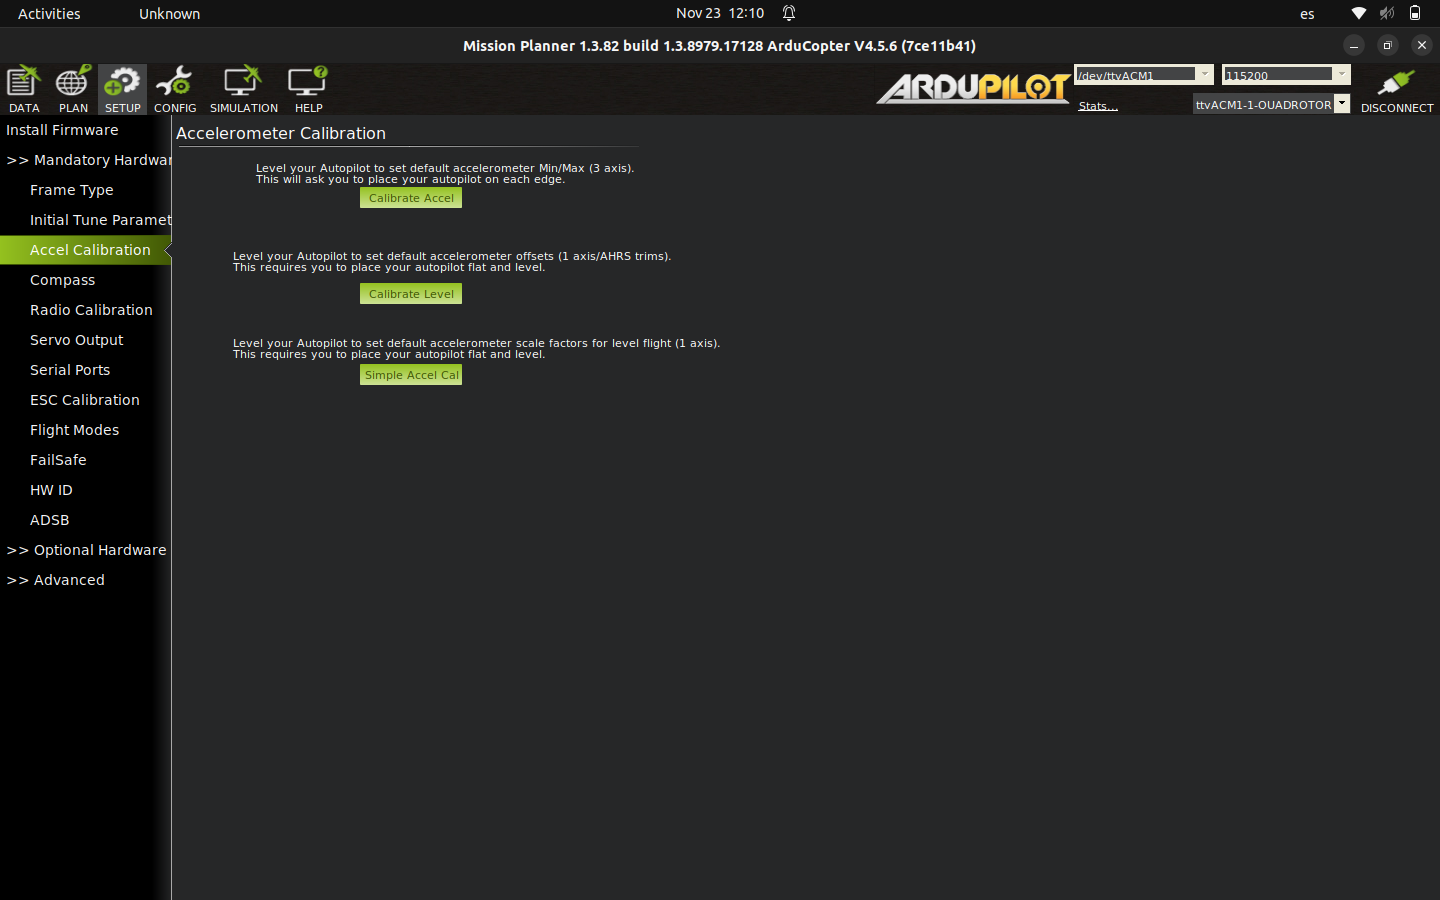
\includegraphics[width=0.8\textwidth]{pictures/mp_calibration.png}
            \caption{Imagen de la configuración de sensores en Mission Planner.}
        \end{figure}

        
        \item \textbf{Parámetros de comunicación:} 
        Para establecer la comunicación entre la Raspberry Pi y el Pixhawk a través de MAVROS y MAVLink, se realizaron los siguientes ajustes en los parámetros utilizando Mission Planner:
        \begin{itemize}
            \item \texttt{SERIAL2\_PROTOCOL}: Configurado en 2 para habilitar MAVLink.
            \item \texttt{SERIAL2\_BAUD}: Ajustado a 921600 para coincidir con la configuración de la Raspberry Pi.
            \item \texttt{SYS\_ID}: Configurado en el ID correspondiente para garantizar una comunicación adecuada con el sistema.
        \end{itemize}
    
    \end{itemize}
    

\section{Sistema de Visión}
\subsection{Especificaciones y Requerimientos} 
El sistema de visión debe cumplir con los siguientes requisitos para garantizar la detección precisa de marcadores Aruco:
    \begin{itemize}
        \item Obtener las matrices de calibración intrínsecas y extrínsecas de la cámara.
        \item Generar y detectar marcadores Aruco de distintos tamaños en tiempo real.
    \end{itemize}

\subsection{Calibración de la Cámara} 
El proceso de calibración de la cámara se realizó utilizando un script en Python con la biblioteca OpenCV. Este procedimiento se detalla a continuación, combinando fragmentos del código y las imágenes obtenidas en cada etapa. El código completo se encuentra en los anexos del documento.
    
    \begin{enumerate}
        \item \textbf{Captura de imágenes:} 
        Se recopilaron múltiples imágenes del tablero de ajedrez desde diferentes ángulos y distancias para abarcar todo el campo de visión de la cámara. Estas imágenes presentaban distorsiones propias de la lente, como se observa en la Figura \ref{fig:imagen_descalibrada}.

        \begin{center}
            \begin{figure}[h!]
                \centering
                %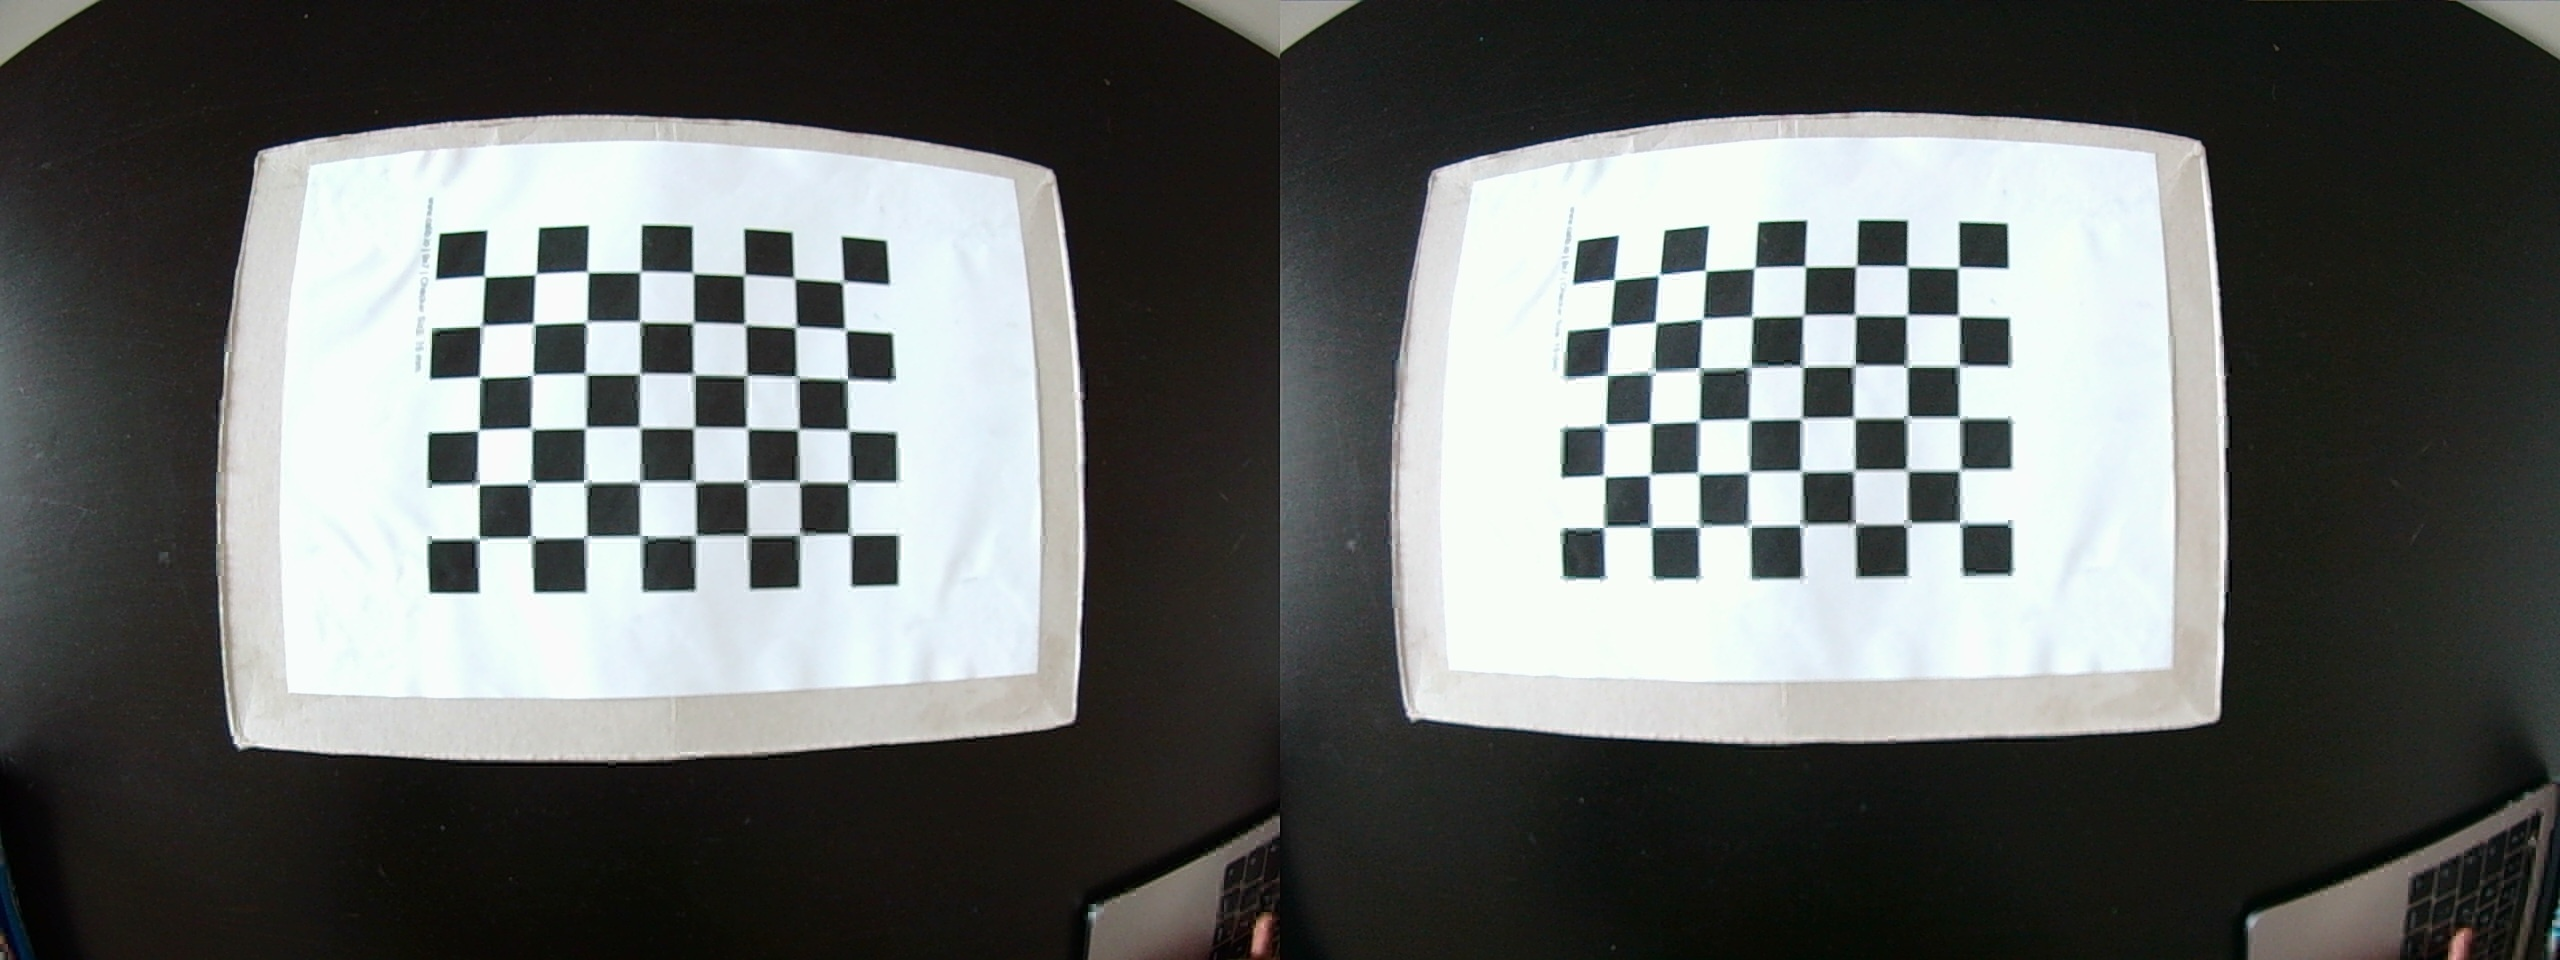
\includegraphics[width=0.8\textwidth]{pictures/imagen_descalibrada.png}
                \caption{Ejemplo de imagen descalibrada tomada durante el proceso de captura.}
                \label{fig:imagen_descalibrada}
            \end{figure}
        \end{center}
    
        \item \textbf{Detección de esquinas:} 
        El script detectó las esquinas internas del tablero de ajedrez mediante la función \texttt{cv2.findChessboardCorners}. Posteriormente, se refinaron las esquinas detectadas utilizando \texttt{cv2.cornerSubPix}, y se visualizaron las líneas superpuestas en las imágenes de calibración, como se muestra en la Figura \ref{fig:det_ejemplos}.
        \begin{verbatim}
        ret, corners = cv2.findChessboardCorners(gray, (ncols, nrows), None)
        corners2 = cv2.cornerSubPix(gray, corners, (11, 11), (-1, -1), criteria)
        \end{verbatim}
        \begin{center}
            \begin{figure}[h!]
                \centering
                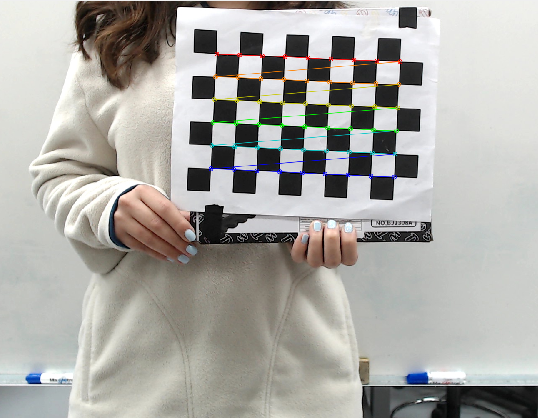
\includegraphics[width=0.8\textwidth]{pictures/calib_predictions.png}
                \caption{Detección y refinamiento de esquinas en el tablero de ajedrez.}
                \label{fig:det_ejemplos}
            \end{figure}
        \end{center}
    
        \item \textbf{Calibración de la cámara:} 
        Utilizando \texttt{cv2.calibrateCamera}, se calcularon los parámetros intrínsecos de la cámara y los coeficientes de distorsión. Estos parámetros permiten corregir las distorsiones en las imágenes capturadas. La Figura \ref{fig:imagen_calibrada} muestra el resultado después de aplicar estos parámetros.
        \begin{verbatim}
        ret, mtx, dist, rvecs, tvecs = cv2.calibrateCamera(objpoints, 
                                                           imgpoints, 
                                                           img_size, 
                                                           None, 
                                                           None)
        \end{verbatim}
        Donde:
        \begin{itemize}
            \item \texttt{mtx}: Matriz intrínseca de la cámara.
            \item \texttt{dist}: Coeficientes de distorsión.
            \item \texttt{rvecs}, \texttt{tvecs}: Rotaciones y traslaciones.
        \end{itemize}
        \begin{center}
            \begin{figure}[h!]
                \centering
                %\includegraphics[width=0.8\textwidth]{pictures/imagen_calibrada.png}
                \caption{Imagen calibrada después de aplicar los parámetros obtenidos.}
                \label{fig:imagen_calibrada}
            \end{figure}
        \end{center}
    
        \item \textbf{Cálculo del error de calibración:} 
        Se verificó la precisión del modelo calculando el error promedio mediante \texttt{cv2.projectPoints}. Este cálculo compara las esquinas detectadas y proyectadas.
        \begin{verbatim}
        error = cv2.norm(imgpoints[i], imgpoints2, cv2.NORM_L2) / len(imgpoints2)
        print("Total error: {}".format(mean_error / len(objpoints)))
        \end{verbatim}
    
        \item \textbf{Almacenamiento de parámetros:} 
        Los parámetros de calibración obtenidos se guardaron en un archivo JSON, lo que permite su reutilización en futuros procesos de corrección de imágenes.
        \begin{verbatim}
        data = {"camera_matrix": mtx.tolist(), 
                "distortion_coefficients": dist.tolist()}
        with open(output_path, "w") as file:
            json.dump(data, file, indent=4)
        \end{verbatim}
    \end{enumerate}
    
    
\subsection{Generación de Marcadores ArUco} 
    Se generaron marcadores ArUco adaptados al sistema, incluyendo tamaños y patrones específicos. En particular, se crearon marcadores embebidos, donde un marcador interno se incrusta dentro de un marcador externo para maximizar la precisión en la detección. A continuación, se describe el proceso paso a paso, destacando las partes importantes del código utilizado. El código completo se encuentra en los anexos del documento.
    
    \begin{enumerate}
        \item \textbf{Carga del diccionario de ArUco:} 
        Se utilizó el diccionario predefinido \texttt{DICT\_6X6\_250} de OpenCV, adecuado para generar marcadores con diferentes patrones y niveles de detalle.
        \begin{verbatim}
        aruco_dict = aruco.getPredefinedDictionary(aruco.DICT_6X6_250)
        \end{verbatim}
    
        \item \textbf{Generación del marcador externo:} 
        Se definió un tamaño de 220 píxeles para el marcador externo (\texttt{outer\_marker\_size}) y se generó el marcador con un ID específico (\texttt{outer\_marker\_id}). Esto permitió crear un marcador grande que sirviera como contenedor.
        \begin{verbatim}
        outer_marker = aruco.generateImageMarker(aruco_dict, 
                                                 outer_marker_id, 
                                                 outer_marker_size)
        \end{verbatim}
        \begin{center}
            \begin{figure}[h!]
                \centering
                
\includegraphics[width=0.4\textwidth]{pictures/aruco_marker_5.png}
                \caption{Marcador ArUco externo generado.}
            \end{figure}
        \end{center}
    
        \item \textbf{Generación del marcador interno:} 
        El marcador interno se generó con un tamaño de 50 píxeles (\texttt{inner\_marker\_size}) y un ID específico (\texttt{inner\_marker\_id}). Este marcador se diseñó para ser incrustado dentro del marcador externo.
        \begin{verbatim}
        inner_marker = aruco.generateImageMarker(aruco_dict, 
                                                 inner_marker_id, 
                                                 inner_marker_size)
        \end{verbatim}

        \begin{center}
            \begin{figure}[h!]
                \centering
                
\includegraphics[width=0.2\textwidth]{pictures/aruco_marker_100.png}
                \caption{Marcador interno con borde blanco añadido.}
            \end{figure}
        \end{center}
    
        \item \textbf{Creación del borde blanco alrededor del marcador interno:} 
        Se añadió un borde blanco de un píxel alrededor del marcador interno utilizando \texttt{cv2.copyMakeBorder}, lo que facilita su incrustación y aumenta la visibilidad en diferentes condiciones de iluminación.
        \begin{verbatim}
        inner_marker_with_border = cv2.copyMakeBorder(
            inner_marker,
            top=border_size,
            bottom=border_size,
            left=border_size,
            right=border_size,
            borderType=cv2.BORDER_CONSTANT,
            value=255  # Blanco
        )
        \end{verbatim}
        
    
        \item \textbf{Incrustación del marcador interno en el marcador externo:} 
        Se calculó la posición central para incrustar el marcador interno con borde en el marcador externo. El marcador externo se modificó para incluir un fondo negro en el centro antes de insertar el marcador interno con borde.
        \begin{verbatim}
        center_position = (outer_marker_size - inner_marker_with_border_size) // 2
        e_aruco_marker[center_position:center_position + inner_marker_with_border_size,
                       center_position:center_position + inner_marker_with_border_size] = 0
        e_aruco_marker[center_position:center_position + inner_marker_with_border_size,
                       center_position:center_position + inner_marker_with_border_size] = inner_marker_with_border
        \end{verbatim}
        \begin{center}
            \begin{figure}[h!]
                \centering
                
\includegraphics[width=0.4\textwidth]{pictures/embedded_aruco.png}
                \caption{Marcador ArUco embebido generado.}
            \end{figure}
        \end{center}
    
        \item \textbf{Almacenamiento del marcador embebido:} 
        Finalmente, el marcador generado se guardó como una imagen PNG para su uso posterior.
        \begin{verbatim}
        cv2.imwrite(f'embedded_aruco_marker_{outer_marker_id}_{inner_marker_id}.png', 
                    e_aruco_marker)
        \end{verbatim}
    \end{enumerate}


\subsection{Detección de Marcadores e-Aruco en Tiempo Real} 
    El sistema fue diseñado para detectar marcadores Aruco en tiempo real, utilizando imágenes capturadas por una cámara conectada al dron. Este proceso se llevó a cabo mediante un nodo en ROS2 que procesa las imágenes y estima la pose de los marcadores con respecto a la cámara. El código completo se encuentra en los anexos del documento. A continuación, se describe el paso a paso del sistema:
    
    \begin{enumerate}
        \item \textbf{Publicación de imágenes desde el dron:} 
        La computadora auxiliar en el dron (companion computer) publica imágenes comprimidas capturadas por la cámara a un tópico de ROS 2 (\texttt{/camera\_image/compressed}). Estas imágenes se envían a la computadora en tierra para su procesamiento.
    
        \item \textbf{Recepción de imágenes en la computadora en tierra:} 
        Un nodo en la computadora en tierra se suscribe a las imágenes publicadas por el dron y realiza las siguientes tareas:
        \begin{itemize}
            \item Convierte las imágenes comprimidas en matrices utilizables para el procesamiento con OpenCV.
            \item Redimensiona las imágenes y las convierte a escala de grises para optimizar la detección.
        \end{itemize}
    
        \item \textbf{Detección de marcadores Aruco:} 
        Se utiliza la biblioteca OpenCV para detectar los marcadores Aruco presentes en la imagen. Los pasos incluyen:
        \begin{itemize}
            \item Uso del diccionario \texttt{DICT\_6X6\_250} para identificar marcadores específicos.
            \item Cálculo de las esquinas de los marcadores detectados mediante \texttt{aruco.detectMarkers}.
            \item Dibujo de los marcadores detectados para su visualización.
        \end{itemize}
        \begin{center}
            \begin{figure}[h!]
                \centering
                %\includegraphics[width=0.8\textwidth]{pictures/deteccion_arucos.png}
                \caption{Detección de marcadores Aruco en la imagen procesada.}
            \end{figure}
        \end{center}
    
        \item \textbf{Estimación de la pose:} 
        Para cada marcador detectado, se calculó su posición y orientación en el espacio con respecto a la cámara. Esto se realizó utilizando la función \texttt{aruco.estimatePoseSingleMarkers}, que devuelve:
        \begin{itemize}
            \item \texttt{tvec}: Vector de traslación (\textit{x}, \textit{y}, \textit{z}) en metros.
            \item \texttt{rvec}: Vector de rotación que se convierte en ángulos de Euler (\textit{roll}, \textit{pitch}, \textit{yaw}) mediante matrices de rotación.
        \end{itemize}
        \begin{center}
            \begin{figure}[h!]
                \centering
                %\includegraphics[width=0.8\textwidth]{pictures/calculo_pose.png}
                \caption{Representación gráfica de la posición y orientación calculada de un marcador Aruco.}
            \end{figure}
        \end{center}
    
        \item \textbf{Visualización y publicación de resultados:} 
        Los resultados obtenidos, incluyendo la pose de los marcadores, se visualizaron en tiempo real y se publicaron en un nuevo tópico de ROS 2 (\texttt{/aruco\_detection/compressed}). Las imágenes procesadas contenían:
        \begin{itemize}
            \item Marcadores detectados con esquinas resaltadas.
            \item Ejes X, Y y Z proyectados para mostrar la orientación de cada marcador.
        \end{itemize}
        \begin{center}
            \begin{figure}[h!]
                \centering
                %\includegraphics[width=0.8\textwidth]{pictures/marcadores_ejes.png}
                \caption{Imagen con marcadores detectados y ejes proyectados.}
            \end{figure}
        \end{center}
    
        \item \textbf{Correcciones de posición:} 
        Basándose en los valores de \texttt{tvec}, se calcularon las correcciones necesarias para ajustar la posición del dron con respecto al marcador, incluyendo movimientos laterales (\textit{x}), verticales (\textit{y}) y de profundidad (\textit{z}).
    
        \item \textbf{Interacción con el sistema:} 
        Los resultados de la detección de marcadores Aruco se utilizaron para visualizar la posición y orientación del drone en tiempo real, lo que permitirá posteriormente que el sistema de control pueda ajustar las mismas para su aterrizaje en la estación de carga.
    \end{enumerate}
    

\section{Sistema de Comunicación}

    \subsection{Especificaciones y Requerimientos} 
    El sistema de comunicación entre el dron y la estación de carga fue diseñado para garantizar la transferencia eficiente y en tiempo real de datos críticos. Los requisitos principales son:
    
    \begin{itemize}
        \item \textbf{Red local basada en WiFi:} 
        Proporcionar una comunicación efectiva entre los dispositivos sin necesidad de acceso a Internet.
        \item \textbf{Middleware DDS de ROS 2:} 
        Utilizar la arquitectura de nodos y tópicos de ROS 2 para gestionar la comunicación de datos entre los dispositivos conectados.
    \end{itemize}
    
    \subsection{Estructura de Comunicación} 
    
    \subsubsection{Red Local WiFi} 
    La red local fue creada utilizando un router WiFi que conecta todos los dispositivos involucrados en el sistema, incluyendo el dron, la estación de carga y la computadora en tierra. Esta configuración eliminó la necesidad de Internet, proporcionando un entorno seguro y aislado para la transmisión de datos. El dron, equipado con una computadora auxiliar, transmitió datos mediante tópicos de ROS 2, como imágenes comprimidas y mensajes de estado, hacia la estación de carga y la computadora en tierra.
    
    \begin{figure}
        \centering
        %\includegraphics[width=0.8\textwidth]{pictures/wifi_network.png}
        \caption{Diagrama de la red local WiFi utilizada en el sistema.}
    \end{figure}
    
    \subsubsection{Comunicación mediante ROS 2} 
    El sistema utilizó la arquitectura de nodos y tópicos de ROS 2 para gestionar la comunicación entre los dispositivos. Cada dispositivo en la red cumplió funciones específicas relacionadas con la publicación y suscripción de datos relevantes:
    
    \begin{itemize}
        \item \textbf{Dron:} 
        Publicó imágenes de la cámara (\texttt{/camera\_image/compressed}) y datos de estado relacionados con la batería, posición y otros parámetros críticos.
        \item \textbf{Computadora en tierra:} 
        Contiene una interfaz que se suscribió a los tópicos publicados por el dron para:
        \begin{itemize}
            \item Procesar imágenes y calcular la posición de los marcadores Aruco.
            \item Mostrar datos de estado del dron, como nivel de batería y modo de vuelo, etc. en tiempo real.
            \item Publicar comandos hacia la estación de carga, como abrir o retraer el cajón de la estación, mediante tópicos específicos.
        \end{itemize}
        \item \textbf{Estación de carga:} 
        Se suscribió a los comandos enviados desde la interfaz de la computadora en tierra para ejecutar las acciones necesarias, como la apertura y cierre del cajón.
    \end{itemize}
    
    \begin{figure}
        \centering
        %\includegraphics[width=0.8\textwidth]{pictures/ros2_comms.png}
        \caption{Diagrama de comunicación entre los dispositivos utilizando ROS 2.}
    \end{figure}
    

    




 % Llama al archivo 'desarrollo.tex' desde la carpeta 'chapters'

\chapter{Results} % Capítulo principal de desarrollo
Este capítulo presenta los resultados obtenidos en el desarrollo y prueba de la base de carga modular y el dron instrumentado para la interacción con la estación de carga. 

\section{Resultados del Diseño y Manufactura de la Base de Carga}
En esta sección se presentan los resultados obtenidos en el diseño y manufactura de la estación de carga y del drone. Se incluyen los resultados de las pruebas de funcionamiento de la estacíon de carga y de las pruebas de vuelo, detección de ArUcos y comunicación entre los diferentes dispositivos.

\subsection{Diseño CAD Final del 1er protopipo de la Estación de Carga}


\subsection{Diseño e Instrumentación del Drone}

\subsection{Movimiento del Cajón}

\subsection{Vuelo del Drone}

\subsection{Carga y Descarga de Batería}

\subsection{Detección del ArUco}

\subsection{Sistema de Comunicación}
Documentación de los tiempos de respuesta, confiabilidad y estabilidad de la comunicación. Las métricas de latencia y tasa de éxito en la transferencia de datos se presentan en gráficos para facilitar el análisis.

\section{Análisis de Desempeño General}
\subsection{Resultados de Integración Global}
Comparación entre el desempeño esperado y el desempeño real en la interacción entre el dron y la estación de carga.
 % Llama al archivo 'resultados.tex' desde la carpeta 'chapters'

\chapter{Conclusions} % Capítulo de conclusiones
In this section, the achievements of the thesis are summarized, from the design and fabrication of the modular charging station to the instrumentation of the drone with localization sensors and a computer vision system. The objectives were successfully met, highlighting the modularity and efficiency of the proposed charging system, as well as the successful integration of the drone with the charging station.

Despite the accomplishments, areas for improvement were identified for future work. Among these enhancements is the implementation of a fast-charging system, which would significantly reduce the drone's charging time. Additionally, developing an autonomous lighting system to ensure precise landing in low-light conditions would improve the drone's operational autonomy in various scenarios.

Finally, optimizing the communication system between the drone and the charging station could increase the efficiency of the landing and charging process, particularly when operating multiple stations in a swarm environment. % Llama al archivo 'conclusiones.tex' desde la carpeta 'chapters'

% Bibliografía
\chapter{Bibliography} % Capítulo de bibliografía
\input{chapters/bibliografía.tex} % Llama al archivo 'bibliografía.tex' desde la carpeta 'chapters'

\end{document}